\documentclass[1p]{elsarticle_modified}
%\bibliographystyle{elsarticle-num}

%\usepackage[colorlinks]{hyperref}
%\usepackage{abbrmath_seonhwa} %\Abb, \Ascr, \Acal ,\Abf, \Afrak
\usepackage{amsfonts}
\usepackage{amssymb}
\usepackage{amsmath}
\usepackage{amsthm}
\usepackage{scalefnt}
\usepackage{amsbsy}
\usepackage{kotex}
\usepackage{caption}
\usepackage{subfig}
\usepackage{color}
\usepackage{graphicx}
\usepackage{xcolor} %% white, black, red, green, blue, cyan, magenta, yellow
\usepackage{float}
\usepackage{setspace}
\usepackage{hyperref}

\usepackage{tikz}
\usetikzlibrary{arrows}

\usepackage{multirow}
\usepackage{array} % fixed length table
\usepackage{hhline}

%%%%%%%%%%%%%%%%%%%%%
\makeatletter
\renewcommand*\env@matrix[1][\arraystretch]{%
	\edef\arraystretch{#1}%
	\hskip -\arraycolsep
	\let\@ifnextchar\new@ifnextchar
	\array{*\c@MaxMatrixCols c}}
\makeatother %https://tex.stackexchange.com/questions/14071/how-can-i-increase-the-line-spacing-in-a-matrix
%%%%%%%%%%%%%%%

\usepackage[normalem]{ulem}

\newcommand{\msout}[1]{\ifmmode\text{\sout{\ensuremath{#1}}}\else\sout{#1}\fi}
%SOURCE: \msout is \stkout macro in https://tex.stackexchange.com/questions/20609/strikeout-in-math-mode

\newcommand{\cancel}[1]{
	\ifmmode
	{\color{red}\msout{#1}}
	\else
	{\color{red}\sout{#1}}
	\fi
}

\newcommand{\add}[1]{
	{\color{blue}\uwave{#1}}
}

\newcommand{\replace}[2]{
	\ifmmode
	{\color{red}\msout{#1}}{\color{blue}\uwave{#2}}
	\else
	{\color{red}\sout{#1}}{\color{blue}\uwave{#2}}
	\fi
}

\newcommand{\Sol}{\mathcal{S}} %segment
\newcommand{\D}{D} %diagram
\newcommand{\A}{\mathcal{A}} %arc


%%%%%%%%%%%%%%%%%%%%%%%%%%%%%5 test

\def\sl{\operatorname{\textup{SL}}(2,\Cbb)}
\def\psl{\operatorname{\textup{PSL}}(2,\Cbb)}
\def\quan{\mkern 1mu \triangleright \mkern 1mu}

\theoremstyle{definition}
\newtheorem{thm}{Theorem}[section]
\newtheorem{prop}[thm]{Proposition}
\newtheorem{lem}[thm]{Lemma}
\newtheorem{ques}[thm]{Question}
\newtheorem{cor}[thm]{Corollary}
\newtheorem{defn}[thm]{Definition}
\newtheorem{exam}[thm]{Example}
\newtheorem{rmk}[thm]{Remark}
\newtheorem{alg}[thm]{Algorithm}

\newcommand{\I}{\sqrt{-1}}
\begin{document}

%\begin{frontmatter}
%
%\title{Boundary parabolic representations of knots up to 8 crossings}
%
%%% Group authors per affiliation:
%\author{Yunhi Cho} 
%\address{Department of Mathematics, University of Seoul, Seoul, Korea}
%\ead{yhcho@uos.ac.kr}
%
%
%\author{Seonhwa Kim} %\fnref{s_kim}}
%\address{Center for Geometry and Physics, Institute for Basic Science, Pohang, 37673, Korea}
%\ead{ryeona17@ibs.re.kr}
%
%\author{Hyuk Kim}
%\address{Department of Mathematical Sciences, Seoul National University, Seoul 08826, Korea}
%\ead{hyukkim@snu.ac.kr}
%
%\author{Seokbeom Yoon}
%\address{Department of Mathematical Sciences, Seoul National University, Seoul, 08826,  Korea}
%\ead{sbyoon15@snu.ac.kr}
%
%\begin{abstract}
%We find all boundary parabolic representation of knots up to 8 crossings.
%
%\end{abstract}
%\begin{keyword}
%    \MSC[2010] 57M25 
%\end{keyword}
%
%\end{frontmatter}

%\linenumbers
%\tableofcontents
%
\newcommand\colored[1]{\textcolor{white}{\rule[-0.35ex]{0.8em}{1.4ex}}\kern-0.8em\color{red} #1}%
%\newcommand\colored[1]{\textcolor{white}{ #1}\kern-2.17ex	\textcolor{white}{ #1}\kern-1.81ex	\textcolor{white}{ #1}\kern-2.15ex\color{red}#1	}

{\Large $\underline{12a_{1019}~(K12a_{1019})}$}

\setlength{\tabcolsep}{10pt}
\renewcommand{\arraystretch}{1.6}
\vspace{1cm}\begin{tabular}{m{100pt}>{\centering\arraybackslash}m{274pt}}
\multirow{5}{120pt}{
	\centering
	\includegraphics[width=112pt]{../../../GIT/diagram.site/Diagrams/png/1820_12a_1019.png}\\
\ \ \ A knot diagram\footnotemark}&
\allowdisplaybreaks
\textbf{Linearized knot diagam} \\
\cline{2-2}
 &
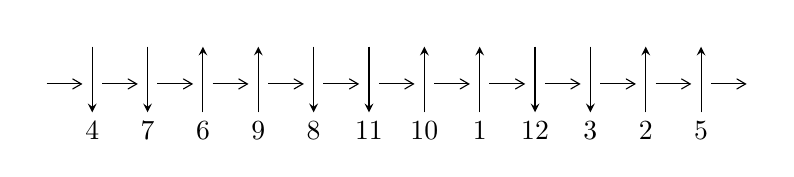
\begin{tikzpicture}[x=20pt, y=17pt]
	% nodes
	\node (C0) at (0, 0) {};
	\node (C1) at (1, 0) {};
	\node (C1U) at (1, +1) {};
	\node (C1D) at (1, -1) {4};

	\node (C2) at (2, 0) {};
	\node (C2U) at (2, +1) {};
	\node (C2D) at (2, -1) {7};

	\node (C3) at (3, 0) {};
	\node (C3U) at (3, +1) {};
	\node (C3D) at (3, -1) {6};

	\node (C4) at (4, 0) {};
	\node (C4U) at (4, +1) {};
	\node (C4D) at (4, -1) {9};

	\node (C5) at (5, 0) {};
	\node (C5U) at (5, +1) {};
	\node (C5D) at (5, -1) {8};

	\node (C6) at (6, 0) {};
	\node (C6U) at (6, +1) {};
	\node (C6D) at (6, -1) {11};

	\node (C7) at (7, 0) {};
	\node (C7U) at (7, +1) {};
	\node (C7D) at (7, -1) {10};

	\node (C8) at (8, 0) {};
	\node (C8U) at (8, +1) {};
	\node (C8D) at (8, -1) {1};

	\node (C9) at (9, 0) {};
	\node (C9U) at (9, +1) {};
	\node (C9D) at (9, -1) {12};

	\node (C10) at (10, 0) {};
	\node (C10U) at (10, +1) {};
	\node (C10D) at (10, -1) {3};

	\node (C11) at (11, 0) {};
	\node (C11U) at (11, +1) {};
	\node (C11D) at (11, -1) {2};

	\node (C12) at (12, 0) {};
	\node (C12U) at (12, +1) {};
	\node (C12D) at (12, -1) {5};
	\node (C13) at (13, 0) {};

	% arrows
	\draw[->,>={angle 60}]
	(C0) edge (C1) (C1) edge (C2) (C2) edge (C3) (C3) edge (C4) (C4) edge (C5) (C5) edge (C6) (C6) edge (C7) (C7) edge (C8) (C8) edge (C9) (C9) edge (C10) (C10) edge (C11) (C11) edge (C12) (C12) edge (C13) ;	\draw[->,>=stealth]
	(C1U) edge (C1D) (C2U) edge (C2D) (C3D) edge (C3U) (C4D) edge (C4U) (C5U) edge (C5D) (C6U) edge (C6D) (C7D) edge (C7U) (C8D) edge (C8U) (C9U) edge (C9D) (C10U) edge (C10D) (C11D) edge (C11U) (C12D) edge (C12U) ;
	\end{tikzpicture} \\
\hhline{~~} \\& 
\textbf{Solving Sequence} \\ \cline{2-2} 
 &
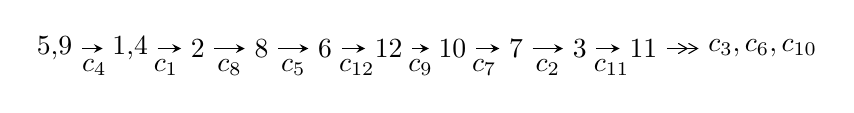
\begin{tikzpicture}[x=23pt, y=7pt]
	% node
	\node (A0) at (-1/8, 0) {5,9};
	\node (A1) at (17/16, 0) {1,4};
	\node (A2) at (17/8, 0) {2};
	\node (A3) at (25/8, 0) {8};
	\node (A4) at (33/8, 0) {6};
	\node (A5) at (41/8, 0) {12};
	\node (A6) at (49/8, 0) {10};
	\node (A7) at (57/8, 0) {7};
	\node (A8) at (65/8, 0) {3};
	\node (A9) at (73/8, 0) {11};
	\node (C1) at (1/2, -1) {$c_{4}$};
	\node (C2) at (13/8, -1) {$c_{1}$};
	\node (C3) at (21/8, -1) {$c_{8}$};
	\node (C4) at (29/8, -1) {$c_{5}$};
	\node (C5) at (37/8, -1) {$c_{12}$};
	\node (C6) at (45/8, -1) {$c_{9}$};
	\node (C7) at (53/8, -1) {$c_{7}$};
	\node (C8) at (61/8, -1) {$c_{2}$};
	\node (C9) at (69/8, -1) {$c_{11}$};
	\node (A10) at (11, 0) {$c_{3},c_{6},c_{10}$};

	% edge
	\draw[->,>=stealth]	
	(A0) edge (A1) (A1) edge (A2) (A2) edge (A3) (A3) edge (A4) (A4) edge (A5) (A5) edge (A6) (A6) edge (A7) (A7) edge (A8) (A8) edge (A9) ;
	\draw[->>,>={angle 60}]	
	(A9) edge (A10);
\end{tikzpicture} \\ 

\end{tabular} \\

\footnotetext{
The image of knot diagram is generated by the software ``\textbf{Draw programme}" developed by Andrew Bartholomew(\url{http://www.layer8.co.uk/maths/draw/index.htm\#Running-draw}), where we modified some parts for our purpose(\url{https://github.com/CATsTAILs/LinksPainter}).
}\phantom \\ \newline 
\centering \textbf{Ideals for irreducible components\footnotemark of $X_{\text{par}}$} 
 
\begin{align*}
I^u_{1}&=\langle 
b+u,\;a-1,\;u^{10}+5 u^9+12 u^8+15 u^7+9 u^6- u^5-3 u^4+u^3+4 u^2+u-1\rangle \\
I^u_{2}&=\langle 
b+u,\;-1.75613\times10^{16} u^{21}+1.11888\times10^{17} u^{20}+\cdots+2.50431\times10^{13} a+1.70131\times10^{16},\\
\phantom{I^u_{2}}&\phantom{= \langle  }5 u^{22}-35 u^{21}+\cdots-6 u+3\rangle \\
I^u_{3}&=\langle 
1.10406\times10^{16} u^{21}-7.03969\times10^{16} u^{20}+\cdots+2.50431\times10^{13} b-1.05368\times10^{16},\;a-1,\\
\phantom{I^u_{3}}&\phantom{= \langle  }5 u^{22}-35 u^{21}+\cdots-6 u+3\rangle \\
I^u_{4}&=\langle 
3.63226\times10^{15} u^{21}+8.27964\times10^{16} u^{20}+\cdots+3.35609\times10^{15} b+3.49818\times10^{17},\\
\phantom{I^u_{4}}&\phantom{= \langle  }8.19885\times10^{15} u^{21}+1.82243\times10^{17} u^{20}+\cdots+1.34244\times10^{16} a+4.80275\times10^{17},\\
\phantom{I^u_{4}}&\phantom{= \langle  }3 u^{22}+72 u^{21}+\cdots+1792 u+512\rangle \\
I^u_{5}&=\langle 
b+u,\;a+1,\;u^{14}-5 u^{13}+12 u^{12}-16 u^{11}+13 u^{10}-8 u^9+8 u^8-9 u^7+6 u^6-3 u^5+3 u^4-3 u^3+u^2+1\rangle \\
I^u_{6}&=\langle 
- u^2+b-1,\;u^3- u^2+a-1,\;u^4- u^3+u^2- u+1\rangle \\
I^u_{7}&=\langle 
b+u,\;- u^3-2 u^2+a- u+1,\;u^4+3 u^3+4 u^2+2 u+1\rangle \\
I^u_{8}&=\langle 
u^3+3 u^2+b+3 u+1,\;a+1,\;u^4+3 u^3+4 u^2+2 u+1\rangle \\
I^u_{9}&=\langle 
-2.18056\times10^{72} u^{53}+2.46832\times10^{73} u^{52}+\cdots+5.29251\times10^{67} b+9.57025\times10^{72},\\
\phantom{I^u_{9}}&\phantom{= \langle  }9.57025\times10^{72} a u^{53}+6.77762\times10^{72} u^{53}+\cdots-4.18369\times10^{73} a-3.12165\times10^{73},\\
\phantom{I^u_{9}}&\phantom{= \langle  }3 u^{54}-36 u^{53}+\cdots-72 u+9\rangle \\
I^u_{10}&=\langle 
b+u,\;a-1,\;u^4+2 u^3+2 u^2+u+1\rangle \\
\end{align*}\\
\begin{align*}
I^u_{11}&=\langle 
3 u^5 a^3-3 u^5 a^2+\cdots+3 a+3,\;-4 u^5 a^3+4 u^5 a^2+\cdots+b-9 a,\\
\phantom{I^u_{11}}&\phantom{= \langle  }u^5 a^3+u^4 a^3- u^5 a^2- u^4 a^2-2 u^3 a^2- a^2 u^2+2 u^3 a+b a u+u^2 b-2 b u+3 a u+a-2 u+1,\\
\phantom{I^u_{11}}&\phantom{= \langle  }u^6 a^3- u^6 a^2+\cdots+a- u,\\
\phantom{I^u_{11}}&\phantom{= \langle  }u^5 a^4+a^4 u^4- u^5 a^3-2 u^4 a^3-2 a^3 u^3+u^4 a^2- a^3 u^2+2 u^3 a^2+2 a^2 u^2+3 a^2 u- u^2 a+a^2-3 a u- a+1\rangle \\
\\
\end{align*}
\raggedright * 10 irreducible components of $\dim_{\mathbb{C}}=0$, with total 214 representations.\\
\raggedright * 1 irreducible components of $\dim_{\mathbb{C}}=1$ \\
\footnotetext{All coefficients of polynomials are rational numbers. But the coefficients are sometimes approximated in decimal forms when there is not enough margin.}
\newpage
\renewcommand{\arraystretch}{1}
\centering \section*{I. $I^u_{1}= \langle b+u,\;a-1,\;u^{10}+5 u^9+\cdots+u-1 \rangle$}
\flushleft \textbf{(i) Arc colorings}\\
\begin{tabular}{m{7pt} m{180pt} m{7pt} m{180pt} }
\flushright $a_{5}=$&$\begin{pmatrix}1\\0\end{pmatrix}$ \\
\flushright $a_{9}=$&$\begin{pmatrix}0\\u\end{pmatrix}$ \\
\flushright $a_{1}=$&$\begin{pmatrix}1\\- u\end{pmatrix}$ \\
\flushright $a_{4}=$&$\begin{pmatrix}1\\u^2\end{pmatrix}$ \\
\flushright $a_{2}=$&$\begin{pmatrix}u^2+u+1\\u^4+u^3- u\end{pmatrix}$ \\
\flushright $a_{8}=$&$\begin{pmatrix}- u\\u^2+u\end{pmatrix}$ \\
\flushright $a_{6}=$&$\begin{pmatrix}- u^3- u^2+1\\u^4+2 u^3+u^2\end{pmatrix}$ \\
\flushright $a_{12}=$&$\begin{pmatrix}u+1\\- u\end{pmatrix}$ \\
\flushright $a_{10}=$&$\begin{pmatrix}- u^3-2 u^2- u\\u^3+u^2+u\end{pmatrix}$ \\
\flushright $a_{7}=$&$\begin{pmatrix}- u^8-4 u^7-7 u^6-6 u^5-2 u^4- u\\u^8+3 u^7+5 u^6+4 u^5+2 u^4+u^2+u\end{pmatrix}$ \\
\flushright $a_{3}=$&$\begin{pmatrix}- u^8-3 u^7-4 u^6- u^5+2 u^4+2 u^3+1\\u^9+4 u^8+7 u^7+6 u^6+2 u^5+u^2\end{pmatrix}$ \\
\flushright $a_{11}=$&$\begin{pmatrix}u^7+3 u^6+5 u^5+4 u^4+2 u^3+u+1\\u^9+3 u^8+4 u^7+u^6-2 u^5-2 u^4- u\end{pmatrix}$\\&\end{tabular}
\flushleft \textbf{(ii) Obstruction class $= -1$}\\~\\
\flushleft \textbf{(iii) Cusp Shapes $= -6 u^9-30 u^8-66 u^7-72 u^6-33 u^5+6 u^4+6 u^3-9 u^2-15 u$}\\~\\
\newpage\renewcommand{\arraystretch}{1}
\flushleft \textbf{(iv) u-Polynomials at the component}\newline \\
\begin{tabular}{m{50pt}|m{274pt}}
Crossings & \hspace{64pt}u-Polynomials at each crossing \\
\hline $$\begin{aligned}c_{1},c_{5},c_{9}\end{aligned}$$&$\begin{aligned}
&u^{10}-4 u^9+9 u^8-11 u^7+8 u^6-7 u^5+10 u^4-13 u^3+3 u^2+6 u-1
\end{aligned}$\\
\hline $$\begin{aligned}c_{2},c_{6},c_{10}\end{aligned}$$&$\begin{aligned}
&u^{10}+5 u^9+12 u^8+15 u^7+9 u^6- u^5-3 u^4+u^3+4 u^2+u-1
\end{aligned}$\\
\hline $$\begin{aligned}c_{3},c_{7},c_{11}\end{aligned}$$&$\begin{aligned}
&u^{10}+4 u^9+9 u^8+11 u^7+8 u^6+7 u^5+10 u^4+13 u^3+3 u^2-6 u-1
\end{aligned}$\\
\hline $$\begin{aligned}c_{4},c_{8},c_{12}\end{aligned}$$&$\begin{aligned}
&u^{10}-5 u^9+12 u^8-15 u^7+9 u^6+u^5-3 u^4- u^3+4 u^2- u-1
\end{aligned}$\\
\hline
\end{tabular}\\~\\
\newpage\renewcommand{\arraystretch}{1}
\flushleft \textbf{(v) Riley Polynomials at the component}\newline \\
\begin{tabular}{m{50pt}|m{274pt}}
Crossings & \hspace{64pt}Riley Polynomials at each crossing \\
\hline $$\begin{aligned}c_{1},c_{3},c_{5}\\c_{7},c_{9},c_{11}\end{aligned}$$&$\begin{aligned}
&y^{10}+2 y^9+\cdots-42 y+1
\end{aligned}$\\
\hline $$\begin{aligned}c_{2},c_{4},c_{6}\\c_{8},c_{10},c_{12}\end{aligned}$$&$\begin{aligned}
&y^{10}- y^9+12 y^8-5 y^7+37 y^6- y^5+29 y^4-41 y^3+20 y^2-9 y+1
\end{aligned}$\\
\hline
\end{tabular}\\~\\
\newpage\flushleft \textbf{(vi) Complex Volumes and Cusp Shapes}
$$\begin{array}{c|c|c}  
\text{Solutions to }I^u_{1}& \I (\text{vol} + \sqrt{-1}CS) & \text{Cusp shape}\\
 \hline 
\begin{aligned}
u &= -0.479749 + 0.993559 I \\
a &= \phantom{-}1.00000\phantom{ +0.000000I} \\
b &= \phantom{-}0.479749 - 0.993559 I\end{aligned}
 & -7.19382 + 6.52036 I & -6.88308 - 3.27411 I \\ \hline\begin{aligned}
u &= -0.479749 - 0.993559 I \\
a &= \phantom{-}1.00000\phantom{ +0.000000I} \\
b &= \phantom{-}0.479749 + 0.993559 I\end{aligned}
 & -7.19382 - 6.52036 I & -6.88308 + 3.27411 I \\ \hline\begin{aligned}
u &= -0.797113\phantom{ +0.000000I} \\
a &= \phantom{-}1.00000\phantom{ +0.000000I} \\
b &= \phantom{-}0.797113\phantom{ +0.000000I}\end{aligned}
 & \phantom{-}1.30949\phantom{ +0.000000I} & \phantom{-}7.15720\phantom{ +0.000000I} \\ \hline\begin{aligned}
u &= \phantom{-}0.548565 + 0.400517 I \\
a &= \phantom{-}1.00000\phantom{ +0.000000I} \\
b &= -0.548565 - 0.400517 I\end{aligned}
 & \phantom{-0.000000 } -3.62072 I & \phantom{-0.000000 -}0. + 2.45070 I \\ \hline\begin{aligned}
u &= \phantom{-}0.548565 - 0.400517 I \\
a &= \phantom{-}1.00000\phantom{ +0.000000I} \\
b &= -0.548565 + 0.400517 I\end{aligned}
 & \phantom{-0.000000 -}3.62072 I & \phantom{-0.000000 } 0. - 2.45070 I \\ \hline\begin{aligned}
u &= -1.17617 + 0.93991 I \\
a &= \phantom{-}1.00000\phantom{ +0.000000I} \\
b &= \phantom{-}1.17617 - 0.93991 I\end{aligned}
 & \phantom{-}7.19382 - 6.52036 I & \phantom{-}6.88308 + 3.27411 I \\ \hline\begin{aligned}
u &= -1.17617 - 0.93991 I \\
a &= \phantom{-}1.00000\phantom{ +0.000000I} \\
b &= \phantom{-}1.17617 + 0.93991 I\end{aligned}
 & \phantom{-}7.19382 + 6.52036 I & \phantom{-}6.88308 - 3.27411 I \\ \hline\begin{aligned}
u &= -1.18492 + 1.08537 I \\
a &= \phantom{-}1.00000\phantom{ +0.000000I} \\
b &= \phantom{-}1.18492 - 1.08537 I\end{aligned}
 & \phantom{-0.000000 } -23.1517 I & \phantom{-0.000000 -}0. + 11.68475 I \\ \hline\begin{aligned}
u &= -1.18492 - 1.08537 I \\
a &= \phantom{-}1.00000\phantom{ +0.000000I} \\
b &= \phantom{-}1.18492 + 1.08537 I\end{aligned}
 & \phantom{-0.000000 -}23.1517 I & \phantom{-0.000000 } 0. - 11.68475 I \\ \hline\begin{aligned}
u &= \phantom{-}0.381661\phantom{ +0.000000I} \\
a &= \phantom{-}1.00000\phantom{ +0.000000I} \\
b &= -0.381661\phantom{ +0.000000I}\end{aligned}
 & -1.30949\phantom{ +0.000000I} & -7.15720\phantom{ +0.000000I}\\
 \hline 
 \end{array}$$\newpage\newpage\renewcommand{\arraystretch}{1}
\centering \section*{II. $I^u_{2}= \langle b+u,\;-1.76\times10^{16} u^{21}+1.12\times10^{17} u^{20}+\cdots+2.50\times10^{13} a+1.70\times10^{16},\;5 u^{22}-35 u^{21}+\cdots-6 u+3 \rangle$}
\flushleft \textbf{(i) Arc colorings}\\
\begin{tabular}{m{7pt} m{180pt} m{7pt} m{180pt} }
\flushright $a_{5}=$&$\begin{pmatrix}1\\0\end{pmatrix}$ \\
\flushright $a_{9}=$&$\begin{pmatrix}0\\u\end{pmatrix}$ \\
\flushright $a_{1}=$&$\begin{pmatrix}701.241 u^{21}-4467.82 u^{20}+\cdots+278.914 u-679.351\\- u\end{pmatrix}$ \\
\flushright $a_{4}=$&$\begin{pmatrix}1\\u^2\end{pmatrix}$ \\
\flushright $a_{2}=$&$\begin{pmatrix}976.258 u^{21}-6219.70 u^{20}+\cdots+388.205 u-943.869\\108.799 u^{21}-692.854 u^{20}+\cdots+41.8787 u-103.945\end{pmatrix}$ \\
\flushright $a_{8}=$&$\begin{pmatrix}1700.33 u^{21}-10820.3 u^{20}+\cdots+771.696 u-1669.95\\275.017 u^{21}-1751.88 u^{20}+\cdots+109.291 u-264.518\end{pmatrix}$ \\
\flushright $a_{6}=$&$\begin{pmatrix}61.3336 u^{21}-372.520 u^{20}+\cdots+149.128 u-102.182\\-77.3231 u^{21}+493.468 u^{20}+\cdots-24.7045 u+72.4263\end{pmatrix}$ \\
\flushright $a_{12}=$&$\begin{pmatrix}701.241 u^{21}-4467.82 u^{20}+\cdots+279.914 u-679.351\\- u\end{pmatrix}$ \\
\flushright $a_{10}=$&$\begin{pmatrix}1150.30 u^{21}-7316.58 u^{20}+\cdots+555.113 u-1140.91\\275.017 u^{21}-1751.88 u^{20}+\cdots+109.291 u-264.518\end{pmatrix}$ \\
\flushright $a_{7}=$&$\begin{pmatrix}202.358 u^{21}-1275.68 u^{20}+\cdots+198.939 u-228.787\\-81.7460 u^{21}+519.761 u^{20}+\cdots-28.5216 u+74.5041\end{pmatrix}$ \\
\flushright $a_{3}=$&$\begin{pmatrix}531.498 u^{21}-3324.09 u^{20}+\cdots+609.330 u-637.060\\19.5456 u^{21}-123.605 u^{20}+\cdots+22.1415 u-23.6804\end{pmatrix}$ \\
\flushright $a_{11}=$&$\begin{pmatrix}-537.954 u^{21}+3428.49 u^{20}+\cdots-168.930 u+494.299\\-137.858 u^{21}+877.769 u^{20}+\cdots-54.1322 u+129.505\end{pmatrix}$\\&\end{tabular}
\flushleft \textbf{(ii) Obstruction class $= -1$}\\~\\
\flushleft \textbf{(iii) Cusp Shapes $= \frac{18316216866445270}{37564710667623} u^{21}-\frac{115678549605691945}{37564710667623} u^{20}+\cdots+\frac{11105532068647541}{37564710667623} u-\frac{1881652730664947}{4173856740847}$}\\~\\
\newpage\renewcommand{\arraystretch}{1}
\flushleft \textbf{(iv) u-Polynomials at the component}\newline \\
\begin{tabular}{m{50pt}|m{274pt}}
Crossings & \hspace{64pt}u-Polynomials at each crossing \\
\hline $$\begin{aligned}c_{1},c_{5}\end{aligned}$$&$\begin{aligned}
&u^{22}+5 u^{21}+\cdots+115 u+55
\end{aligned}$\\
\hline $$\begin{aligned}c_{2}\end{aligned}$$&$\begin{aligned}
&3(3 u^{22}+72 u^{21}+\cdots+1792 u+512)
\end{aligned}$\\
\hline $$\begin{aligned}c_{3}\end{aligned}$$&$\begin{aligned}
&75(75 u^{22}+1875 u^{21}+\cdots+3211264 u+262144)
\end{aligned}$\\
\hline $$\begin{aligned}c_{4},c_{12}\end{aligned}$$&$\begin{aligned}
&5(5 u^{22}+35 u^{21}+\cdots+6 u+3)
\end{aligned}$\\
\hline $$\begin{aligned}c_{6},c_{10}\end{aligned}$$&$\begin{aligned}
&5(5 u^{22}-35 u^{21}+\cdots-6 u+3)
\end{aligned}$\\
\hline $$\begin{aligned}c_{7},c_{11}\end{aligned}$$&$\begin{aligned}
&u^{22}-5 u^{21}+\cdots-115 u+55
\end{aligned}$\\
\hline $$\begin{aligned}c_{8}\end{aligned}$$&$\begin{aligned}
&3(3 u^{22}-72 u^{21}+\cdots-1792 u+512)
\end{aligned}$\\
\hline $$\begin{aligned}c_{9}\end{aligned}$$&$\begin{aligned}
&75(75 u^{22}-1875 u^{21}+\cdots-3211264 u+262144)
\end{aligned}$\\
\hline
\end{tabular}\\~\\
\newpage\renewcommand{\arraystretch}{1}
\flushleft \textbf{(v) Riley Polynomials at the component}\newline \\
\begin{tabular}{m{50pt}|m{274pt}}
Crossings & \hspace{64pt}Riley Polynomials at each crossing \\
\hline $$\begin{aligned}c_{1},c_{5},c_{7}\\c_{11}\end{aligned}$$&$\begin{aligned}
&y^{22}+11 y^{21}+\cdots+20875 y+3025
\end{aligned}$\\
\hline $$\begin{aligned}c_{2},c_{8}\end{aligned}$$&$\begin{aligned}
&9(9 y^{22}-84 y^{21}+\cdots+9371648 y+262144)
\end{aligned}$\\
\hline $$\begin{aligned}c_{3},c_{9}\end{aligned}$$&$\begin{aligned}
&5625\\
&\cdot(5625 y^{22}-33375 y^{21}+\cdots-184683593728 y+68719476736)
\end{aligned}$\\
\hline $$\begin{aligned}c_{4},c_{6},c_{10}\\c_{12}\end{aligned}$$&$\begin{aligned}
&25(25 y^{22}+25 y^{21}+\cdots-174 y+9)
\end{aligned}$\\
\hline
\end{tabular}\\~\\
\newpage\flushleft \textbf{(vi) Complex Volumes and Cusp Shapes}
$$\begin{array}{c|c|c}  
\text{Solutions to }I^u_{2}& \I (\text{vol} + \sqrt{-1}CS) & \text{Cusp shape}\\
 \hline 
\begin{aligned}
u &= -0.424422 + 0.935543 I \\
a &= \phantom{-}1.44492 + 0.96232 I \\
b &= \phantom{-}0.424422 - 0.935543 I\end{aligned}
 & -3.80225 - 13.36980 I & -4.78895 + 11.87368 I \\ \hline\begin{aligned}
u &= -0.424422 - 0.935543 I \\
a &= \phantom{-}1.44492 - 0.96232 I \\
b &= \phantom{-}0.424422 + 0.935543 I\end{aligned}
 & -3.80225 + 13.36980 I & -4.78895 - 11.87368 I \\ \hline\begin{aligned}
u &= -0.846187 + 0.332900 I \\
a &= \phantom{-}1.75108 - 0.39745 I \\
b &= \phantom{-}0.846187 - 0.332900 I\end{aligned}
 & \phantom{-}3.78801 - 0.96344 I & \phantom{-}9.72237 + 2.09748 I \\ \hline\begin{aligned}
u &= -0.846187 - 0.332900 I \\
a &= \phantom{-}1.75108 + 0.39745 I \\
b &= \phantom{-}0.846187 + 0.332900 I\end{aligned}
 & \phantom{-}3.78801 + 0.96344 I & \phantom{-}9.72237 - 2.09748 I \\ \hline\begin{aligned}
u &= \phantom{-}0.449611 + 0.993975 I \\
a &= -0.272885 - 0.146365 I \\
b &= -0.449611 - 0.993975 I\end{aligned}
 & -3.78801 - 0.96344 I & -9.72237 + 2.09748 I \\ \hline\begin{aligned}
u &= \phantom{-}0.449611 - 0.993975 I \\
a &= -0.272885 + 0.146365 I \\
b &= -0.449611 + 0.993975 I\end{aligned}
 & -3.78801 + 0.96344 I & -9.72237 - 2.09748 I \\ \hline\begin{aligned}
u &= \phantom{-}0.634038 + 0.993177 I \\
a &= -0.819199 - 0.140629 I \\
b &= -0.634038 - 0.993177 I\end{aligned}
 & -5.93206 + 1.93386 I & -15.6328 - 1.6122 I \\ \hline\begin{aligned}
u &= \phantom{-}0.634038 - 0.993177 I \\
a &= -0.819199 + 0.140629 I \\
b &= -0.634038 + 0.993177 I\end{aligned}
 & -5.93206 - 1.93386 I & -15.6328 + 1.6122 I \\ \hline\begin{aligned}
u &= -0.536047 + 1.061394 I \\
a &= \phantom{-}0.127085 - 0.174072 I \\
b &= \phantom{-}0.536047 - 1.061394 I\end{aligned}
 & -3.40489 - 7.87661 I & -4.97285 + 6.45494 I \\ \hline\begin{aligned}
u &= -0.536047 - 1.061394 I \\
a &= \phantom{-}0.127085 + 0.174072 I \\
b &= \phantom{-}0.536047 + 1.061394 I\end{aligned}
 & -3.40489 + 7.87661 I & -4.97285 - 6.45494 I\\
 \hline 
 \end{array}$$\newpage$$\begin{array}{c|c|c}  
\text{Solutions to }I^u_{2}& \I (\text{vol} + \sqrt{-1}CS) & \text{Cusp shape}\\
 \hline 
\begin{aligned}
u &= \phantom{-}0.629786 + 0.256221 I \\
a &= -1.13406 + 2.82964 I \\
b &= -0.629786 - 0.256221 I\end{aligned}
 & -0.44414 + 14.02510 I & \phantom{-}4.9360 - 14.4554 I \\ \hline\begin{aligned}
u &= \phantom{-}0.629786 - 0.256221 I \\
a &= -1.13406 - 2.82964 I \\
b &= -0.629786 + 0.256221 I\end{aligned}
 & -0.44414 - 14.02510 I & \phantom{-}4.9360 + 14.4554 I \\ \hline\begin{aligned}
u &= \phantom{-}1.113808 + 0.776539 I \\
a &= -1.163157 - 0.177259 I \\
b &= -1.113808 - 0.776539 I\end{aligned}
 & \phantom{-}3.40489 + 7.87661 I & \phantom{-}4.97285 - 6.45494 I \\ \hline\begin{aligned}
u &= \phantom{-}1.113808 - 0.776539 I \\
a &= -1.163157 + 0.177259 I \\
b &= -1.113808 + 0.776539 I\end{aligned}
 & \phantom{-}3.40489 - 7.87661 I & \phantom{-}4.97285 + 6.45494 I \\ \hline\begin{aligned}
u &= \phantom{-}0.628680 + 0.002790 I \\
a &= -1.93746 + 2.37902 I \\
b &= -0.628680 - 0.002790 I\end{aligned}
 & \phantom{-}5.93206 - 1.93386 I & \phantom{-}15.6328 + 1.6122 I \\ \hline\begin{aligned}
u &= \phantom{-}0.628680 - 0.002790 I \\
a &= -1.93746 - 2.37902 I \\
b &= -0.628680 + 0.002790 I\end{aligned}
 & \phantom{-}5.93206 + 1.93386 I & \phantom{-}15.6328 - 1.6122 I \\ \hline\begin{aligned}
u &= \phantom{-}1.12956 + 1.03672 I \\
a &= -1.082565 + 0.004380 I \\
b &= -1.12956 - 1.03672 I\end{aligned}
 & \phantom{-}0.44414 + 14.02510 I & -4.9360 - 14.4554 I \\ \hline\begin{aligned}
u &= \phantom{-}1.12956 - 1.03672 I \\
a &= -1.082565 - 0.004380 I \\
b &= -1.12956 + 1.03672 I\end{aligned}
 & \phantom{-}0.44414 - 14.02510 I & -4.9360 + 14.4554 I \\ \hline\begin{aligned}
u &= \phantom{-}1.11352 + 1.07627 I \\
a &= -0.980300 + 0.178884 I \\
b &= -1.11352 - 1.07627 I\end{aligned}
 & \phantom{-}3.80225 + 13.36980 I & \phantom{-}4.78895 - 11.87368 I \\ \hline\begin{aligned}
u &= \phantom{-}1.11352 - 1.07627 I \\
a &= -0.980300 - 0.178884 I \\
b &= -1.11352 + 1.07627 I\end{aligned}
 & \phantom{-}3.80225 - 13.36980 I & \phantom{-}4.78895 + 11.87368 I\\
 \hline 
 \end{array}$$\newpage$$\begin{array}{c|c|c}  
\text{Solutions to }I^u_{2}& \I (\text{vol} + \sqrt{-1}CS) & \text{Cusp shape}\\
 \hline 
\begin{aligned}
u &= -0.392344 + 0.032218 I \\
a &= \phantom{-}6.89988 - 4.45942 I \\
b &= \phantom{-}0.392344 - 0.032218 I\end{aligned}
 & \phantom{-0.000000 -}3.92307 I & \phantom{-0.000000 } 0. - 11.69335 I \\ \hline\begin{aligned}
u &= -0.392344 - 0.032218 I \\
a &= \phantom{-}6.89988 + 4.45942 I \\
b &= \phantom{-}0.392344 + 0.032218 I\end{aligned}
 & \phantom{-0.000000 } -3.92307 I & \phantom{-0.000000 -}0. + 11.69335 I\\
 \hline 
 \end{array}$$\newpage\newpage\renewcommand{\arraystretch}{1}
\centering \section*{III. $I^u_{3}= \langle 1.10\times10^{16} u^{21}-7.04\times10^{16} u^{20}+\cdots+2.50\times10^{13} b-1.05\times10^{16},\;a-1,\;5 u^{22}-35 u^{21}+\cdots-6 u+3 \rangle$}
\flushleft \textbf{(i) Arc colorings}\\
\begin{tabular}{m{7pt} m{180pt} m{7pt} m{180pt} }
\flushright $a_{5}=$&$\begin{pmatrix}1\\0\end{pmatrix}$ \\
\flushright $a_{9}=$&$\begin{pmatrix}0\\u\end{pmatrix}$ \\
\flushright $a_{1}=$&$\begin{pmatrix}1\\-440.863 u^{21}+2811.02 u^{20}+\cdots-162.138 u+420.745\end{pmatrix}$ \\
\flushright $a_{4}=$&$\begin{pmatrix}1\\u^2\end{pmatrix}$ \\
\flushright $a_{2}=$&$\begin{pmatrix}440.863 u^{21}-2811.02 u^{20}+\cdots+162.138 u-419.745\\-267.622 u^{21}+1707.14 u^{20}+\cdots-96.6350 u+255.734\end{pmatrix}$ \\
\flushright $a_{8}=$&$\begin{pmatrix}- u\\275.017 u^{21}-1751.88 u^{20}+\cdots+109.291 u-264.518\end{pmatrix}$ \\
\flushright $a_{6}=$&$\begin{pmatrix}-173.241 u^{21}+1103.89 u^{20}+\cdots-65.5030 u+166.010\\-77.3231 u^{21}+493.468 u^{20}+\cdots-24.7045 u+72.4263\end{pmatrix}$ \\
\flushright $a_{12}=$&$\begin{pmatrix}440.863 u^{21}-2811.02 u^{20}+\cdots+162.138 u-419.745\\-440.863 u^{21}+2811.02 u^{20}+\cdots-162.138 u+420.745\end{pmatrix}$ \\
\flushright $a_{10}=$&$\begin{pmatrix}120.710 u^{21}-767.650 u^{20}+\cdots+60.5867 u-120.148\\-395.728 u^{21}+2519.53 u^{20}+\cdots-168.878 u+384.666\end{pmatrix}$ \\
\flushright $a_{7}=$&$\begin{pmatrix}-39.4674 u^{21}+256.726 u^{20}+\cdots+14.2498 u+25.2194\\-35.2420 u^{21}+218.436 u^{20}+\cdots-38.3921 u+41.1163\end{pmatrix}$ \\
\flushright $a_{3}=$&$\begin{pmatrix}215.842 u^{21}-1373.04 u^{20}+\cdots+90.6322 u-204.878\\106.519 u^{21}-678.178 u^{20}+\cdots+37.8759 u-99.8725\end{pmatrix}$ \\
\flushright $a_{11}=$&$\begin{pmatrix}-124.174 u^{21}+787.469 u^{20}+\cdots-60.6488 u+120.487\\-110.111 u^{21}+704.990 u^{20}+\cdots-26.5354 u+101.718\end{pmatrix}$\\&\end{tabular}
\flushleft \textbf{(ii) Obstruction class $= -1$}\\~\\
\flushleft \textbf{(iii) Cusp Shapes $= \frac{18316216866445270}{37564710667623} u^{21}-\frac{115678549605691945}{37564710667623} u^{20}+\cdots+\frac{11105532068647541}{37564710667623} u-\frac{1881652730664947}{4173856740847}$}\\~\\
\newpage\renewcommand{\arraystretch}{1}
\flushleft \textbf{(iv) u-Polynomials at the component}\newline \\
\begin{tabular}{m{50pt}|m{274pt}}
Crossings & \hspace{64pt}u-Polynomials at each crossing \\
\hline $$\begin{aligned}c_{1}\end{aligned}$$&$\begin{aligned}
&75(75 u^{22}-1875 u^{21}+\cdots-3211264 u+262144)
\end{aligned}$\\
\hline $$\begin{aligned}c_{2},c_{10}\end{aligned}$$&$\begin{aligned}
&5(5 u^{22}-35 u^{21}+\cdots-6 u+3)
\end{aligned}$\\
\hline $$\begin{aligned}c_{3},c_{11}\end{aligned}$$&$\begin{aligned}
&u^{22}-5 u^{21}+\cdots-115 u+55
\end{aligned}$\\
\hline $$\begin{aligned}c_{4},c_{8}\end{aligned}$$&$\begin{aligned}
&5(5 u^{22}+35 u^{21}+\cdots+6 u+3)
\end{aligned}$\\
\hline $$\begin{aligned}c_{5},c_{9}\end{aligned}$$&$\begin{aligned}
&u^{22}+5 u^{21}+\cdots+115 u+55
\end{aligned}$\\
\hline $$\begin{aligned}c_{6}\end{aligned}$$&$\begin{aligned}
&3(3 u^{22}+72 u^{21}+\cdots+1792 u+512)
\end{aligned}$\\
\hline $$\begin{aligned}c_{7}\end{aligned}$$&$\begin{aligned}
&75(75 u^{22}+1875 u^{21}+\cdots+3211264 u+262144)
\end{aligned}$\\
\hline $$\begin{aligned}c_{12}\end{aligned}$$&$\begin{aligned}
&3(3 u^{22}-72 u^{21}+\cdots-1792 u+512)
\end{aligned}$\\
\hline
\end{tabular}\\~\\
\newpage\renewcommand{\arraystretch}{1}
\flushleft \textbf{(v) Riley Polynomials at the component}\newline \\
\begin{tabular}{m{50pt}|m{274pt}}
Crossings & \hspace{64pt}Riley Polynomials at each crossing \\
\hline $$\begin{aligned}c_{1},c_{7}\end{aligned}$$&$\begin{aligned}
&5625\\
&\cdot(5625 y^{22}-33375 y^{21}+\cdots-184683593728 y+68719476736)
\end{aligned}$\\
\hline $$\begin{aligned}c_{2},c_{4},c_{8}\\c_{10}\end{aligned}$$&$\begin{aligned}
&25(25 y^{22}+25 y^{21}+\cdots-174 y+9)
\end{aligned}$\\
\hline $$\begin{aligned}c_{3},c_{5},c_{9}\\c_{11}\end{aligned}$$&$\begin{aligned}
&y^{22}+11 y^{21}+\cdots+20875 y+3025
\end{aligned}$\\
\hline $$\begin{aligned}c_{6},c_{12}\end{aligned}$$&$\begin{aligned}
&9(9 y^{22}-84 y^{21}+\cdots+9371648 y+262144)
\end{aligned}$\\
\hline
\end{tabular}\\~\\
\newpage\flushleft \textbf{(vi) Complex Volumes and Cusp Shapes}
$$\begin{array}{c|c|c}  
\text{Solutions to }I^u_{3}& \I (\text{vol} + \sqrt{-1}CS) & \text{Cusp shape}\\
 \hline 
\begin{aligned}
u &= -0.424422 + 0.935543 I \\
a &= \phantom{-}1.00000\phantom{ +0.000000I} \\
b &= \phantom{-}1.51354 - 0.94335 I\end{aligned}
 & -3.80225 - 13.36980 I & -4.78895 + 11.87368 I \\ \hline\begin{aligned}
u &= -0.424422 - 0.935543 I \\
a &= \phantom{-}1.00000\phantom{ +0.000000I} \\
b &= \phantom{-}1.51354 + 0.94335 I\end{aligned}
 & -3.80225 + 13.36980 I & -4.78895 - 11.87368 I \\ \hline\begin{aligned}
u &= -0.846187 + 0.332900 I \\
a &= \phantom{-}1.00000\phantom{ +0.000000I} \\
b &= \phantom{-}1.34943 - 0.91925 I\end{aligned}
 & \phantom{-}3.78801 - 0.96344 I & \phantom{-}9.72237 + 2.09748 I \\ \hline\begin{aligned}
u &= -0.846187 - 0.332900 I \\
a &= \phantom{-}1.00000\phantom{ +0.000000I} \\
b &= \phantom{-}1.34943 + 0.91925 I\end{aligned}
 & \phantom{-}3.78801 + 0.96344 I & \phantom{-}9.72237 - 2.09748 I \\ \hline\begin{aligned}
u &= \phantom{-}0.449611 + 0.993975 I \\
a &= \phantom{-}1.00000\phantom{ +0.000000I} \\
b &= -0.022791 + 0.337049 I\end{aligned}
 & -3.78801 - 0.96344 I & -9.72237 + 2.09748 I \\ \hline\begin{aligned}
u &= \phantom{-}0.449611 - 0.993975 I \\
a &= \phantom{-}1.00000\phantom{ +0.000000I} \\
b &= -0.022791 - 0.337049 I\end{aligned}
 & -3.78801 + 0.96344 I & -9.72237 - 2.09748 I \\ \hline\begin{aligned}
u &= \phantom{-}0.634038 + 0.993177 I \\
a &= \phantom{-}1.00000\phantom{ +0.000000I} \\
b &= \phantom{-}0.379734 + 0.902774 I\end{aligned}
 & -5.93206 + 1.93386 I & -15.6328 - 1.6122 I \\ \hline\begin{aligned}
u &= \phantom{-}0.634038 - 0.993177 I \\
a &= \phantom{-}1.00000\phantom{ +0.000000I} \\
b &= \phantom{-}0.379734 - 0.902774 I\end{aligned}
 & -5.93206 - 1.93386 I & -15.6328 + 1.6122 I \\ \hline\begin{aligned}
u &= -0.536047 + 1.061394 I \\
a &= \phantom{-}1.00000\phantom{ +0.000000I} \\
b &= -0.116635 - 0.228199 I\end{aligned}
 & -3.40489 - 7.87661 I & -4.97285 + 6.45494 I \\ \hline\begin{aligned}
u &= -0.536047 - 1.061394 I \\
a &= \phantom{-}1.00000\phantom{ +0.000000I} \\
b &= -0.116635 + 0.228199 I\end{aligned}
 & -3.40489 + 7.87661 I & -4.97285 - 6.45494 I\\
 \hline 
 \end{array}$$\newpage$$\begin{array}{c|c|c}  
\text{Solutions to }I^u_{3}& \I (\text{vol} + \sqrt{-1}CS) & \text{Cusp shape}\\
 \hline 
\begin{aligned}
u &= \phantom{-}0.629786 + 0.256221 I \\
a &= \phantom{-}1.00000\phantom{ +0.000000I} \\
b &= \phantom{-}1.43923 - 1.49150 I\end{aligned}
 & -0.44414 + 14.02510 I & \phantom{-}4.9360 - 14.4554 I \\ \hline\begin{aligned}
u &= \phantom{-}0.629786 - 0.256221 I \\
a &= \phantom{-}1.00000\phantom{ +0.000000I} \\
b &= \phantom{-}1.43923 + 1.49150 I\end{aligned}
 & -0.44414 - 14.02510 I & \phantom{-}4.9360 + 14.4554 I \\ \hline\begin{aligned}
u &= \phantom{-}1.113808 + 0.776539 I \\
a &= \phantom{-}1.00000\phantom{ +0.000000I} \\
b &= \phantom{-}1.15789 + 1.10067 I\end{aligned}
 & \phantom{-}3.40489 + 7.87661 I & \phantom{-}4.97285 - 6.45494 I \\ \hline\begin{aligned}
u &= \phantom{-}1.113808 - 0.776539 I \\
a &= \phantom{-}1.00000\phantom{ +0.000000I} \\
b &= \phantom{-}1.15789 - 1.10067 I\end{aligned}
 & \phantom{-}3.40489 - 7.87661 I & \phantom{-}4.97285 + 6.45494 I \\ \hline\begin{aligned}
u &= \phantom{-}0.628680 + 0.002790 I \\
a &= \phantom{-}1.00000\phantom{ +0.000000I} \\
b &= \phantom{-}1.22468 - 1.49024 I\end{aligned}
 & \phantom{-}5.93206 - 1.93386 I & \phantom{-}15.6328 + 1.6122 I \\ \hline\begin{aligned}
u &= \phantom{-}0.628680 - 0.002790 I \\
a &= \phantom{-}1.00000\phantom{ +0.000000I} \\
b &= \phantom{-}1.22468 + 1.49024 I\end{aligned}
 & \phantom{-}5.93206 + 1.93386 I & \phantom{-}15.6328 - 1.6122 I \\ \hline\begin{aligned}
u &= \phantom{-}1.12956 + 1.03672 I \\
a &= \phantom{-}1.00000\phantom{ +0.000000I} \\
b &= \phantom{-}1.22736 + 1.11737 I\end{aligned}
 & \phantom{-}0.44414 + 14.02510 I & -4.9360 - 14.4554 I \\ \hline\begin{aligned}
u &= \phantom{-}1.12956 - 1.03672 I \\
a &= \phantom{-}1.00000\phantom{ +0.000000I} \\
b &= \phantom{-}1.22736 - 1.11737 I\end{aligned}
 & \phantom{-}0.44414 - 14.02510 I & -4.9360 + 14.4554 I \\ \hline\begin{aligned}
u &= \phantom{-}1.11352 + 1.07627 I \\
a &= \phantom{-}1.00000\phantom{ +0.000000I} \\
b &= \phantom{-}1.28411 + 0.85588 I\end{aligned}
 & \phantom{-}3.80225 + 13.36980 I & \phantom{-}4.78895 - 11.87368 I \\ \hline\begin{aligned}
u &= \phantom{-}1.11352 - 1.07627 I \\
a &= \phantom{-}1.00000\phantom{ +0.000000I} \\
b &= \phantom{-}1.28411 - 0.85588 I\end{aligned}
 & \phantom{-}3.80225 - 13.36980 I & \phantom{-}4.78895 + 11.87368 I\\
 \hline 
 \end{array}$$\newpage$$\begin{array}{c|c|c}  
\text{Solutions to }I^u_{3}& \I (\text{vol} + \sqrt{-1}CS) & \text{Cusp shape}\\
 \hline 
\begin{aligned}
u &= -0.392344 + 0.032218 I \\
a &= \phantom{-}1.00000\phantom{ +0.000000I} \\
b &= \phantom{-}2.56345 - 1.97192 I\end{aligned}
 & \phantom{-0.000000 -}3.92307 I & \phantom{-0.000000 } 0. - 11.69335 I \\ \hline\begin{aligned}
u &= -0.392344 - 0.032218 I \\
a &= \phantom{-}1.00000\phantom{ +0.000000I} \\
b &= \phantom{-}2.56345 + 1.97192 I\end{aligned}
 & \phantom{-0.000000 } -3.92307 I & \phantom{-0.000000 -}0. + 11.69335 I\\
 \hline 
 \end{array}$$\newpage\newpage\renewcommand{\arraystretch}{1}
\centering \section*{IV. $I^u_{4}= \langle 3.63\times10^{15} u^{21}+8.28\times10^{16} u^{20}+\cdots+3.36\times10^{15} b+3.50\times10^{17},\;8.20\times10^{15} u^{21}+1.82\times10^{17} u^{20}+\cdots+1.34\times10^{16} a+4.80\times10^{17},\;3 u^{22}+72 u^{21}+\cdots+1792 u+512 \rangle$}
\flushleft \textbf{(i) Arc colorings}\\
\begin{tabular}{m{7pt} m{180pt} m{7pt} m{180pt} }
\flushright $a_{5}=$&$\begin{pmatrix}1\\0\end{pmatrix}$ \\
\flushright $a_{9}=$&$\begin{pmatrix}0\\u\end{pmatrix}$ \\
\flushright $a_{1}=$&$\begin{pmatrix}-0.610745 u^{21}-13.5756 u^{20}+\cdots-133.759 u-35.7764\\-1.08229 u^{21}-24.6705 u^{20}+\cdots-329.042 u-104.234\end{pmatrix}$ \\
\flushright $a_{4}=$&$\begin{pmatrix}1\\u^2\end{pmatrix}$ \\
\flushright $a_{2}=$&$\begin{pmatrix}-0.832932 u^{21}-19.6028 u^{20}+\cdots-346.972 u-116.254\\1.37731 u^{21}+29.6426 u^{20}+\cdots+123.865 u+14.3337\end{pmatrix}$ \\
\flushright $a_{8}=$&$\begin{pmatrix}0.320221 u^{21}+7.51486 u^{20}+\cdots+113.953 u+45.4949\\0.170429 u^{21}+4.56439 u^{20}+\cdots+146.784 u+54.6510\end{pmatrix}$ \\
\flushright $a_{6}=$&$\begin{pmatrix}-0.661396 u^{21}-14.5522 u^{20}+\cdots-140.067 u-42.3997\\-0.847192 u^{21}-20.2905 u^{20}+\cdots-398.826 u-141.965\end{pmatrix}$ \\
\flushright $a_{12}=$&$\begin{pmatrix}0.471546 u^{21}+11.0949 u^{20}+\cdots+195.283 u+68.4574\\-1.08229 u^{21}-24.6705 u^{20}+\cdots-329.042 u-104.234\end{pmatrix}$ \\
\flushright $a_{10}=$&$\begin{pmatrix}-0.494738 u^{21}-11.1459 u^{20}+\cdots-130.462 u-34.7206\\0.644530 u^{21}+14.0964 u^{20}+\cdots+99.6319 u+25.5645\end{pmatrix}$ \\
\flushright $a_{7}=$&$\begin{pmatrix}-0.846816 u^{21}-18.4961 u^{20}+\cdots-64.3540 u-11.3598\\-0.103089 u^{21}-4.25329 u^{20}+\cdots-328.016 u-120.337\end{pmatrix}$ \\
\flushright $a_{3}=$&$\begin{pmatrix}0.0288036 u^{21}+0.643679 u^{20}+\cdots-41.9611 u-8.87420\\-0.100826 u^{21}-3.30811 u^{20}+\cdots-158.801 u-61.2026\end{pmatrix}$ \\
\flushright $a_{11}=$&$\begin{pmatrix}-1.01615 u^{21}-24.2331 u^{20}+\cdots-490.561 u-163.035\\1.98464 u^{21}+42.4414 u^{20}+\cdots+97.8266 u-16.0462\end{pmatrix}$\\&\end{tabular}
\flushleft \textbf{(ii) Obstruction class $= -1$}\\~\\
\flushleft \textbf{(iii) Cusp Shapes $= -\frac{57173920307444841}{16780442909704000} u^{21}-\frac{25170067340752893}{335608858194080} u^{20}+\cdots-\frac{160655803191745028}{262194420464125} u-\frac{48126678289140558}{262194420464125}$}\\~\\
\newpage\renewcommand{\arraystretch}{1}
\flushleft \textbf{(iv) u-Polynomials at the component}\newline \\
\begin{tabular}{m{50pt}|m{274pt}}
Crossings & \hspace{64pt}u-Polynomials at each crossing \\
\hline $$\begin{aligned}c_{1},c_{9}\end{aligned}$$&$\begin{aligned}
&u^{22}+5 u^{21}+\cdots+115 u+55
\end{aligned}$\\
\hline $$\begin{aligned}c_{2},c_{6}\end{aligned}$$&$\begin{aligned}
&5(5 u^{22}-35 u^{21}+\cdots-6 u+3)
\end{aligned}$\\
\hline $$\begin{aligned}c_{3},c_{7}\end{aligned}$$&$\begin{aligned}
&u^{22}-5 u^{21}+\cdots-115 u+55
\end{aligned}$\\
\hline $$\begin{aligned}c_{4}\end{aligned}$$&$\begin{aligned}
&3(3 u^{22}-72 u^{21}+\cdots-1792 u+512)
\end{aligned}$\\
\hline $$\begin{aligned}c_{5}\end{aligned}$$&$\begin{aligned}
&75(75 u^{22}-1875 u^{21}+\cdots-3211264 u+262144)
\end{aligned}$\\
\hline $$\begin{aligned}c_{8},c_{12}\end{aligned}$$&$\begin{aligned}
&5(5 u^{22}+35 u^{21}+\cdots+6 u+3)
\end{aligned}$\\
\hline $$\begin{aligned}c_{10}\end{aligned}$$&$\begin{aligned}
&3(3 u^{22}+72 u^{21}+\cdots+1792 u+512)
\end{aligned}$\\
\hline $$\begin{aligned}c_{11}\end{aligned}$$&$\begin{aligned}
&75(75 u^{22}+1875 u^{21}+\cdots+3211264 u+262144)
\end{aligned}$\\
\hline
\end{tabular}\\~\\
\newpage\renewcommand{\arraystretch}{1}
\flushleft \textbf{(v) Riley Polynomials at the component}\newline \\
\begin{tabular}{m{50pt}|m{274pt}}
Crossings & \hspace{64pt}Riley Polynomials at each crossing \\
\hline $$\begin{aligned}c_{1},c_{3},c_{7}\\c_{9}\end{aligned}$$&$\begin{aligned}
&y^{22}+11 y^{21}+\cdots+20875 y+3025
\end{aligned}$\\
\hline $$\begin{aligned}c_{2},c_{6},c_{8}\\c_{12}\end{aligned}$$&$\begin{aligned}
&25(25 y^{22}+25 y^{21}+\cdots-174 y+9)
\end{aligned}$\\
\hline $$\begin{aligned}c_{4},c_{10}\end{aligned}$$&$\begin{aligned}
&9(9 y^{22}-84 y^{21}+\cdots+9371648 y+262144)
\end{aligned}$\\
\hline $$\begin{aligned}c_{5},c_{11}\end{aligned}$$&$\begin{aligned}
&5625\\
&\cdot(5625 y^{22}-33375 y^{21}+\cdots-184683593728 y+68719476736)
\end{aligned}$\\
\hline
\end{tabular}\\~\\
\newpage\flushleft \textbf{(vi) Complex Volumes and Cusp Shapes}
$$\begin{array}{c|c|c}  
\text{Solutions to }I^u_{4}& \I (\text{vol} + \sqrt{-1}CS) & \text{Cusp shape}\\
 \hline 
\begin{aligned}
u &= -0.379734 + 0.902774 I \\
a &= -1.185761 - 0.203556 I \\
b &= -0.634038 + 0.993177 I\end{aligned}
 & -5.93206 - 1.93386 I & -15.6328 + 1.6122 I \\ \hline\begin{aligned}
u &= -0.379734 - 0.902774 I \\
a &= -1.185761 + 0.203556 I \\
b &= -0.634038 - 0.993177 I\end{aligned}
 & -5.93206 + 1.93386 I & -15.6328 - 1.6122 I \\ \hline\begin{aligned}
u &= -1.28411 + 0.85588 I \\
a &= -0.987222 + 0.180147 I \\
b &= -1.11352 + 1.07627 I\end{aligned}
 & \phantom{-}3.80225 - 13.36980 I & \phantom{-0.000000 -}0. + 11.87368 I \\ \hline\begin{aligned}
u &= -1.28411 - 0.85588 I \\
a &= -0.987222 - 0.180147 I \\
b &= -1.11352 - 1.07627 I\end{aligned}
 & \phantom{-}3.80225 + 13.36980 I & \phantom{-0.000000 } 0. - 11.87368 I \\ \hline\begin{aligned}
u &= -1.15789 + 1.10067 I \\
a &= -0.840216 - 0.128044 I \\
b &= -1.113808 + 0.776539 I\end{aligned}
 & \phantom{-}3.40489 - 7.87661 I & \phantom{-0.000000 } 0 \\ \hline\begin{aligned}
u &= -1.15789 - 1.10067 I \\
a &= -0.840216 + 0.128044 I \\
b &= -1.113808 - 0.776539 I\end{aligned}
 & \phantom{-}3.40489 + 7.87661 I & \phantom{-0.000000 } 0 \\ \hline\begin{aligned}
u &= -1.34943 + 0.91925 I \\
a &= \phantom{-}0.543096 + 0.123269 I \\
b &= \phantom{-}0.846187 - 0.332900 I\end{aligned}
 & \phantom{-}3.78801 - 0.96344 I & \phantom{-0.000000 } 0 \\ \hline\begin{aligned}
u &= -1.34943 - 0.91925 I \\
a &= \phantom{-}0.543096 - 0.123269 I \\
b &= \phantom{-}0.846187 + 0.332900 I\end{aligned}
 & \phantom{-}3.78801 + 0.96344 I & \phantom{-0.000000 } 0 \\ \hline\begin{aligned}
u &= -1.22736 + 1.11737 I \\
a &= -0.923717 + 0.003737 I \\
b &= -1.12956 + 1.03672 I\end{aligned}
 & \phantom{-}0.44414 - 14.02510 I & \phantom{-0.000000 } 0 \\ \hline\begin{aligned}
u &= -1.22736 - 1.11737 I \\
a &= -0.923717 - 0.003737 I \\
b &= -1.12956 - 1.03672 I\end{aligned}
 & \phantom{-}0.44414 + 14.02510 I & \phantom{-0.000000 } 0\\
 \hline 
 \end{array}$$\newpage$$\begin{array}{c|c|c}  
\text{Solutions to }I^u_{4}& \I (\text{vol} + \sqrt{-1}CS) & \text{Cusp shape}\\
 \hline 
\begin{aligned}
u &= \phantom{-}0.022791 + 0.337049 I \\
a &= -2.84584 - 1.52640 I \\
b &= -0.449611 + 0.993975 I\end{aligned}
 & -3.78801 + 0.96344 I & -9.72237 - 2.09748 I \\ \hline\begin{aligned}
u &= \phantom{-}0.022791 - 0.337049 I \\
a &= -2.84584 + 1.52640 I \\
b &= -0.449611 - 0.993975 I\end{aligned}
 & -3.78801 - 0.96344 I & -9.72237 + 2.09748 I \\ \hline\begin{aligned}
u &= \phantom{-}0.116635 + 0.228199 I \\
a &= \phantom{-}2.73586 + 3.74737 I \\
b &= \phantom{-}0.536047 - 1.061394 I\end{aligned}
 & -3.40489 - 7.87661 I & -4.97285 + 6.45494 I \\ \hline\begin{aligned}
u &= \phantom{-}0.116635 - 0.228199 I \\
a &= \phantom{-}2.73586 - 3.74737 I \\
b &= \phantom{-}0.536047 + 1.061394 I\end{aligned}
 & -3.40489 + 7.87661 I & -4.97285 - 6.45494 I \\ \hline\begin{aligned}
u &= -1.51354 + 0.94335 I \\
a &= \phantom{-}0.479427 - 0.319300 I \\
b &= \phantom{-}0.424422 - 0.935543 I\end{aligned}
 & -3.80225 - 13.36980 I & \phantom{-0.000000 } 0 \\ \hline\begin{aligned}
u &= -1.51354 - 0.94335 I \\
a &= \phantom{-}0.479427 + 0.319300 I \\
b &= \phantom{-}0.424422 + 0.935543 I\end{aligned}
 & -3.80225 + 13.36980 I & \phantom{-0.000000 } 0 \\ \hline\begin{aligned}
u &= -1.22468 + 1.49024 I \\
a &= -0.205817 - 0.252725 I \\
b &= -0.628680 - 0.002790 I\end{aligned}
 & \phantom{-}5.93206 - 1.93386 I & \phantom{-0.000000 } 0 \\ \hline\begin{aligned}
u &= -1.22468 - 1.49024 I \\
a &= -0.205817 + 0.252725 I \\
b &= -0.628680 + 0.002790 I\end{aligned}
 & \phantom{-}5.93206 + 1.93386 I & \phantom{-0.000000 } 0 \\ \hline\begin{aligned}
u &= -1.43923 + 1.49150 I \\
a &= -0.122034 - 0.304493 I \\
b &= -0.629786 - 0.256221 I\end{aligned}
 & -0.44414 + 14.02510 I & \phantom{-0.000000 } 0 \\ \hline\begin{aligned}
u &= -1.43923 - 1.49150 I \\
a &= -0.122034 + 0.304493 I \\
b &= -0.629786 + 0.256221 I\end{aligned}
 & -0.44414 - 14.02510 I & \phantom{-0.000000 } 0\\
 \hline 
 \end{array}$$\newpage$$\begin{array}{c|c|c}  
\text{Solutions to }I^u_{4}& \I (\text{vol} + \sqrt{-1}CS) & \text{Cusp shape}\\
 \hline 
\begin{aligned}
u &= -2.56345 + 1.97192 I \\
a &= \phantom{-}0.1022284 + 0.0660707 I \\
b &= \phantom{-}0.392344 - 0.032218 I\end{aligned}
 & \phantom{-0.000000 -}3.92307 I & \phantom{-0.000000 } 0 \\ \hline\begin{aligned}
u &= -2.56345 - 1.97192 I \\
a &= \phantom{-}0.1022284 - 0.0660707 I \\
b &= \phantom{-}0.392344 + 0.032218 I\end{aligned}
 & \phantom{-0.000000 } -3.92307 I & \phantom{-0.000000 } 0\\
 \hline 
 \end{array}$$\newpage\newpage\renewcommand{\arraystretch}{1}
\centering \section*{V. $I^u_{5}= \langle b+u,\;a+1,\;u^{14}-5 u^{13}+\cdots+u^2+1 \rangle$}
\flushleft \textbf{(i) Arc colorings}\\
\begin{tabular}{m{7pt} m{180pt} m{7pt} m{180pt} }
\flushright $a_{5}=$&$\begin{pmatrix}1\\0\end{pmatrix}$ \\
\flushright $a_{9}=$&$\begin{pmatrix}0\\u\end{pmatrix}$ \\
\flushright $a_{1}=$&$\begin{pmatrix}-1\\- u\end{pmatrix}$ \\
\flushright $a_{4}=$&$\begin{pmatrix}1\\u^2\end{pmatrix}$ \\
\flushright $a_{2}=$&$\begin{pmatrix}- u^2+u-1\\- u^4+u^3- u\end{pmatrix}$ \\
\flushright $a_{8}=$&$\begin{pmatrix}- u\\- u^2+u\end{pmatrix}$ \\
\flushright $a_{6}=$&$\begin{pmatrix}u^3- u^2+1\\u^4-2 u^3+u^2\end{pmatrix}$ \\
\flushright $a_{12}=$&$\begin{pmatrix}u-1\\- u\end{pmatrix}$ \\
\flushright $a_{10}=$&$\begin{pmatrix}- u^3+2 u^2- u\\u^3- u^2+u\end{pmatrix}$ \\
\flushright $a_{7}=$&$\begin{pmatrix}u^8-4 u^7+7 u^6-6 u^5+2 u^4- u\\- u^8+3 u^7-5 u^6+4 u^5-2 u^4- u^2+u\end{pmatrix}$ \\
\flushright $a_{3}=$&$\begin{pmatrix}- u^8+3 u^7-4 u^6+u^5+2 u^4-2 u^3+1\\- u^9+4 u^8-7 u^7+6 u^6-2 u^5+u^2\end{pmatrix}$ \\
\flushright $a_{11}=$&$\begin{pmatrix}u^7-3 u^6+5 u^5-4 u^4+2 u^3+u-1\\u^9-3 u^8+4 u^7- u^6-2 u^5+2 u^4- u\end{pmatrix}$\\&\end{tabular}
\flushleft \textbf{(ii) Obstruction class $= 1$}\\~\\
\flushleft \textbf{(iii) Cusp Shapes $= 3 u^{13}-21 u^{12}+60 u^{11}-93 u^{10}+75 u^9-27 u^8+9 u^7-27 u^6+21 u^5+3 u^4-3 u^3-9 u^2+3 u+6$}\\~\\
\newpage\renewcommand{\arraystretch}{1}
\flushleft \textbf{(iv) u-Polynomials at the component}\newline \\
\begin{tabular}{m{50pt}|m{274pt}}
Crossings & \hspace{64pt}u-Polynomials at each crossing \\
\hline $$\begin{aligned}c_{1},c_{5},c_{9}\end{aligned}$$&$\begin{aligned}
&u^{14}-4 u^{13}+\cdots-2 u+1
\end{aligned}$\\
\hline $$\begin{aligned}c_{2},c_{6},c_{10}\end{aligned}$$&$\begin{aligned}
&u^{14}+5 u^{13}+\cdots+u^2+1
\end{aligned}$\\
\hline $$\begin{aligned}c_{3},c_{7},c_{11}\end{aligned}$$&$\begin{aligned}
&u^{14}+4 u^{13}+\cdots+2 u+1
\end{aligned}$\\
\hline $$\begin{aligned}c_{4},c_{8},c_{12}\end{aligned}$$&$\begin{aligned}
&u^{14}-5 u^{13}+\cdots+u^2+1
\end{aligned}$\\
\hline
\end{tabular}\\~\\
\newpage\renewcommand{\arraystretch}{1}
\flushleft \textbf{(v) Riley Polynomials at the component}\newline \\
\begin{tabular}{m{50pt}|m{274pt}}
Crossings & \hspace{64pt}Riley Polynomials at each crossing \\
\hline $$\begin{aligned}c_{1},c_{3},c_{5}\\c_{7},c_{9},c_{11}\end{aligned}$$&$\begin{aligned}
&y^{14}+4 y^{13}+\cdots+24 y+1
\end{aligned}$\\
\hline $$\begin{aligned}c_{2},c_{4},c_{6}\\c_{8},c_{10},c_{12}\end{aligned}$$&$\begin{aligned}
&y^{14}- y^{13}+\cdots+2 y+1
\end{aligned}$\\
\hline
\end{tabular}\\~\\
\newpage\flushleft \textbf{(vi) Complex Volumes and Cusp Shapes}
$$\begin{array}{c|c|c}  
\text{Solutions to }I^u_{5}& \I (\text{vol} + \sqrt{-1}CS) & \text{Cusp shape}\\
 \hline 
\begin{aligned}
u &= \phantom{-}0.582376 + 0.920079 I \\
a &= -1.00000\phantom{ +0.000000I} \\
b &= -0.582376 - 0.920079 I\end{aligned}
 & -4.87762 + 2.24155 I & -5.71062 - 4.08315 I \\ \hline\begin{aligned}
u &= \phantom{-}0.582376 - 0.920079 I \\
a &= -1.00000\phantom{ +0.000000I} \\
b &= -0.582376 + 0.920079 I\end{aligned}
 & -4.87762 - 2.24155 I & -5.71062 + 4.08315 I \\ \hline\begin{aligned}
u &= \phantom{-}1.080860 + 0.257141 I \\
a &= -1.00000\phantom{ +0.000000I} \\
b &= -1.080860 - 0.257141 I\end{aligned}
 & \phantom{-}1.97436 + 7.13139 I & \phantom{-}5.73836 - 7.19904 I \\ \hline\begin{aligned}
u &= \phantom{-}1.080860 - 0.257141 I \\
a &= -1.00000\phantom{ +0.000000I} \\
b &= -1.080860 + 0.257141 I\end{aligned}
 & \phantom{-}1.97436 - 7.13139 I & \phantom{-}5.73836 + 7.19904 I \\ \hline\begin{aligned}
u &= -0.631419 + 0.425056 I \\
a &= -1.00000\phantom{ +0.000000I} \\
b &= \phantom{-}0.631419 - 0.425056 I\end{aligned}
 & -1.19637 + 13.10040 I & -1.00584 - 7.21157 I \\ \hline\begin{aligned}
u &= -0.631419 - 0.425056 I \\
a &= -1.00000\phantom{ +0.000000I} \\
b &= \phantom{-}0.631419 + 0.425056 I\end{aligned}
 & -1.19637 - 13.10040 I & -1.00584 + 7.21157 I \\ \hline\begin{aligned}
u &= -0.220218 + 0.697336 I \\
a &= -1.00000\phantom{ +0.000000I} \\
b &= \phantom{-}0.220218 - 0.697336 I\end{aligned}
 & \phantom{-0.000000 } -4.24748 I & \phantom{-0.000000 -}0. + 7.94314 I \\ \hline\begin{aligned}
u &= -0.220218 - 0.697336 I \\
a &= -1.00000\phantom{ +0.000000I} \\
b &= \phantom{-}0.220218 + 0.697336 I\end{aligned}
 & \phantom{-0.000000 -}4.24748 I & \phantom{-0.000000 } 0. - 7.94314 I \\ \hline\begin{aligned}
u &= -0.427969 + 0.558421 I \\
a &= -1.00000\phantom{ +0.000000I} \\
b &= \phantom{-}0.427969 - 0.558421 I\end{aligned}
 & \phantom{-}4.87762 - 2.24155 I & \phantom{-}5.71062 + 4.08315 I \\ \hline\begin{aligned}
u &= -0.427969 - 0.558421 I \\
a &= -1.00000\phantom{ +0.000000I} \\
b &= \phantom{-}0.427969 + 0.558421 I\end{aligned}
 & \phantom{-}4.87762 + 2.24155 I & \phantom{-}5.71062 - 4.08315 I\\
 \hline 
 \end{array}$$\newpage$$\begin{array}{c|c|c}  
\text{Solutions to }I^u_{5}& \I (\text{vol} + \sqrt{-1}CS) & \text{Cusp shape}\\
 \hline 
\begin{aligned}
u &= \phantom{-}0.958798 + 0.953720 I \\
a &= -1.00000\phantom{ +0.000000I} \\
b &= -0.958798 - 0.953720 I\end{aligned}
 & -1.97436 + 7.13139 I & -5.73836 - 7.19904 I \\ \hline\begin{aligned}
u &= \phantom{-}0.958798 - 0.953720 I \\
a &= -1.00000\phantom{ +0.000000I} \\
b &= -0.958798 + 0.953720 I\end{aligned}
 & -1.97436 - 7.13139 I & -5.73836 + 7.19904 I \\ \hline\begin{aligned}
u &= \phantom{-}1.15757 + 1.04690 I \\
a &= -1.00000\phantom{ +0.000000I} \\
b &= -1.15757 - 1.04690 I\end{aligned}
 & \phantom{-}1.19637 + 13.10040 I & \phantom{-}1.00584 - 7.21157 I \\ \hline\begin{aligned}
u &= \phantom{-}1.15757 - 1.04690 I \\
a &= -1.00000\phantom{ +0.000000I} \\
b &= -1.15757 + 1.04690 I\end{aligned}
 & \phantom{-}1.19637 - 13.10040 I & \phantom{-}1.00584 + 7.21157 I\\
 \hline 
 \end{array}$$\newpage\newpage\renewcommand{\arraystretch}{1}
\centering \section*{VI. $I^u_{6}= \langle - u^2+b-1,\;u^3- u^2+a-1,\;u^4- u^3+u^2- u+1 \rangle$}
\flushleft \textbf{(i) Arc colorings}\\
\begin{tabular}{m{7pt} m{180pt} m{7pt} m{180pt} }
\flushright $a_{5}=$&$\begin{pmatrix}1\\0\end{pmatrix}$ \\
\flushright $a_{9}=$&$\begin{pmatrix}0\\u\end{pmatrix}$ \\
\flushright $a_{1}=$&$\begin{pmatrix}- u^3+u^2+1\\u^2+1\end{pmatrix}$ \\
\flushright $a_{4}=$&$\begin{pmatrix}1\\u^2\end{pmatrix}$ \\
\flushright $a_{2}=$&$\begin{pmatrix}u\\u^2- u+1\end{pmatrix}$ \\
\flushright $a_{8}=$&$\begin{pmatrix}- u^2- u-1\\- u^3- u^2\end{pmatrix}$ \\
\flushright $a_{6}=$&$\begin{pmatrix}4 u^3- u^2+2 u-2\\u^3- u^2-3\end{pmatrix}$ \\
\flushright $a_{12}=$&$\begin{pmatrix}- u^3\\u^2+1\end{pmatrix}$ \\
\flushright $a_{10}=$&$\begin{pmatrix}u^2\\u^3- u^2+u-1\end{pmatrix}$ \\
\flushright $a_{7}=$&$\begin{pmatrix}u^3- u^2- u-1\\- u^3- u^2-1\end{pmatrix}$ \\
\flushright $a_{3}=$&$\begin{pmatrix}3 u^3-2 u^2+2 u-3\\-2 u-1\end{pmatrix}$ \\
\flushright $a_{11}=$&$\begin{pmatrix}-3 u^3+u^2- u+1\\2\end{pmatrix}$\\&\end{tabular}
\flushleft \textbf{(ii) Obstruction class $= 1$}\\~\\
\flushleft \textbf{(iii) Cusp Shapes $= -9 u^3-7 u^2-2 u+1$}\\~\\
\newpage\renewcommand{\arraystretch}{1}
\flushleft \textbf{(iv) u-Polynomials at the component}\newline \\
\begin{tabular}{m{50pt}|m{274pt}}
Crossings & \hspace{64pt}u-Polynomials at each crossing \\
\hline $$\begin{aligned}c_{1},c_{9},c_{10}\end{aligned}$$&$\begin{aligned}
&u^4+u^3+u^2+u+1
\end{aligned}$\\
\hline $$\begin{aligned}c_{2},c_{6}\end{aligned}$$&$\begin{aligned}
&u^4-3 u^3+4 u^2-2 u+1
\end{aligned}$\\
\hline $$\begin{aligned}c_{3},c_{4},c_{7}\end{aligned}$$&$\begin{aligned}
&u^4- u^3+u^2- u+1
\end{aligned}$\\
\hline $$\begin{aligned}c_{5},c_{11}\end{aligned}$$&$\begin{aligned}
&u^4+5 u^2+5
\end{aligned}$\\
\hline $$\begin{aligned}c_{8},c_{12}\end{aligned}$$&$\begin{aligned}
&u^4+3 u^3+4 u^2+2 u+1
\end{aligned}$\\
\hline
\end{tabular}\\~\\
\newpage\renewcommand{\arraystretch}{1}
\flushleft \textbf{(v) Riley Polynomials at the component}\newline \\
\begin{tabular}{m{50pt}|m{274pt}}
Crossings & \hspace{64pt}Riley Polynomials at each crossing \\
\hline $$\begin{aligned}c_{1},c_{3},c_{4}\\c_{7},c_{9},c_{10}\end{aligned}$$&$\begin{aligned}
&y^4+y^3+y^2+y+1
\end{aligned}$\\
\hline $$\begin{aligned}c_{2},c_{6},c_{8}\\c_{12}\end{aligned}$$&$\begin{aligned}
&y^4- y^3+6 y^2+4 y+1
\end{aligned}$\\
\hline $$\begin{aligned}c_{5},c_{11}\end{aligned}$$&$\begin{aligned}
&(y^2+5 y+5)^2
\end{aligned}$\\
\hline
\end{tabular}\\~\\
\newpage\flushleft \textbf{(vi) Complex Volumes and Cusp Shapes}
$$\begin{array}{c|c|c}  
\text{Solutions to }I^u_{6}& \I (\text{vol} + \sqrt{-1}CS) & \text{Cusp shape}\\
 \hline 
\begin{aligned}
u &= -0.309017 + 0.951057 I \\
a &= -0.618034\phantom{ +0.000000I} \\
b &= \phantom{-}0.190983 - 0.587785 I\end{aligned}
 & \phantom{-0.000000 } -4.25078 I & \phantom{-0.000000 -}0. + 7.50245 I \\ \hline\begin{aligned}
u &= -0.309017 - 0.951057 I \\
a &= -0.618034\phantom{ +0.000000I} \\
b &= \phantom{-}0.190983 + 0.587785 I\end{aligned}
 & \phantom{-0.000000 -}4.25078 I & \phantom{-0.000000 } 0. - 7.50245 I \\ \hline\begin{aligned}
u &= \phantom{-}0.809017 + 0.587785 I \\
a &= \phantom{-}1.61803\phantom{ +0.000000I} \\
b &= \phantom{-}1.30902 + 0.95106 I\end{aligned}
 & \phantom{-0.000000 -}9.97355 I & \phantom{-0.000000 } 0. - 16.3925 I \\ \hline\begin{aligned}
u &= \phantom{-}0.809017 - 0.587785 I \\
a &= \phantom{-}1.61803\phantom{ +0.000000I} \\
b &= \phantom{-}1.30902 - 0.95106 I\end{aligned}
 & \phantom{-0.000000 } -9.97355 I & \phantom{-0.000000 -}0. + 16.3925 I\\
 \hline 
 \end{array}$$\newpage\newpage\renewcommand{\arraystretch}{1}
\centering \section*{VII. $I^u_{7}= \langle b+u,\;- u^3-2 u^2+a- u+1,\;u^4+3 u^3+4 u^2+2 u+1 \rangle$}
\flushleft \textbf{(i) Arc colorings}\\
\begin{tabular}{m{7pt} m{180pt} m{7pt} m{180pt} }
\flushright $a_{5}=$&$\begin{pmatrix}1\\0\end{pmatrix}$ \\
\flushright $a_{9}=$&$\begin{pmatrix}0\\u\end{pmatrix}$ \\
\flushright $a_{1}=$&$\begin{pmatrix}u^3+2 u^2+u-1\\- u\end{pmatrix}$ \\
\flushright $a_{4}=$&$\begin{pmatrix}1\\u^2\end{pmatrix}$ \\
\flushright $a_{2}=$&$\begin{pmatrix}u^3+3 u^2+3 u\\- u^3-3 u^2-3 u-1\end{pmatrix}$ \\
\flushright $a_{8}=$&$\begin{pmatrix}- u^3-3 u^2-4 u-1\\u^2+2 u+1\end{pmatrix}$ \\
\flushright $a_{6}=$&$\begin{pmatrix}- u^3-2 u^2- u+2\\u^3+2 u^2+2 u\end{pmatrix}$ \\
\flushright $a_{12}=$&$\begin{pmatrix}u^3+2 u^2+2 u-1\\- u\end{pmatrix}$ \\
\flushright $a_{10}=$&$\begin{pmatrix}-2 u^3-5 u^2-6 u-3\\u^3+u^2+2 u+1\end{pmatrix}$ \\
\flushright $a_{7}=$&$\begin{pmatrix}-3 u^3-7 u^2-6 u\\2 u^3+4 u^2+4 u+1\end{pmatrix}$ \\
\flushright $a_{3}=$&$\begin{pmatrix}2 u^3+6 u^2+8 u+4\\- u^3-2 u^2-3 u-2\end{pmatrix}$ \\
\flushright $a_{11}=$&$\begin{pmatrix}- u^2-2 u-3\\1\end{pmatrix}$\\&\end{tabular}
\flushleft \textbf{(ii) Obstruction class $= 1$}\\~\\
\flushleft \textbf{(iii) Cusp Shapes $= 7 u^3+12 u^2+19 u+6$}\\~\\
\newpage\renewcommand{\arraystretch}{1}
\flushleft \textbf{(iv) u-Polynomials at the component}\newline \\
\begin{tabular}{m{50pt}|m{274pt}}
Crossings & \hspace{64pt}u-Polynomials at each crossing \\
\hline $$\begin{aligned}c_{1},c_{2},c_{5}\end{aligned}$$&$\begin{aligned}
&u^4+u^3+u^2+u+1
\end{aligned}$\\
\hline $$\begin{aligned}c_{3},c_{9}\end{aligned}$$&$\begin{aligned}
&u^4+5 u^2+5
\end{aligned}$\\
\hline $$\begin{aligned}c_{4},c_{12}\end{aligned}$$&$\begin{aligned}
&u^4+3 u^3+4 u^2+2 u+1
\end{aligned}$\\
\hline $$\begin{aligned}c_{6},c_{10}\end{aligned}$$&$\begin{aligned}
&u^4-3 u^3+4 u^2-2 u+1
\end{aligned}$\\
\hline $$\begin{aligned}c_{7},c_{8},c_{11}\end{aligned}$$&$\begin{aligned}
&u^4- u^3+u^2- u+1
\end{aligned}$\\
\hline
\end{tabular}\\~\\
\newpage\renewcommand{\arraystretch}{1}
\flushleft \textbf{(v) Riley Polynomials at the component}\newline \\
\begin{tabular}{m{50pt}|m{274pt}}
Crossings & \hspace{64pt}Riley Polynomials at each crossing \\
\hline $$\begin{aligned}c_{1},c_{2},c_{5}\\c_{7},c_{8},c_{11}\end{aligned}$$&$\begin{aligned}
&y^4+y^3+y^2+y+1
\end{aligned}$\\
\hline $$\begin{aligned}c_{3},c_{9}\end{aligned}$$&$\begin{aligned}
&(y^2+5 y+5)^2
\end{aligned}$\\
\hline $$\begin{aligned}c_{4},c_{6},c_{10}\\c_{12}\end{aligned}$$&$\begin{aligned}
&y^4- y^3+6 y^2+4 y+1
\end{aligned}$\\
\hline
\end{tabular}\\~\\
\newpage\flushleft \textbf{(vi) Complex Volumes and Cusp Shapes}
$$\begin{array}{c|c|c}  
\text{Solutions to }I^u_{7}& \I (\text{vol} + \sqrt{-1}CS) & \text{Cusp shape}\\
 \hline 
\begin{aligned}
u &= -0.190983 + 0.587785 I \\
a &= -1.61803\phantom{ +0.000000I} \\
b &= \phantom{-}0.190983 - 0.587785 I\end{aligned}
 & \phantom{-0.000000 } -4.25078 I & \phantom{-0.000000 -}0. + 7.50245 I \\ \hline\begin{aligned}
u &= -0.190983 - 0.587785 I \\
a &= -1.61803\phantom{ +0.000000I} \\
b &= \phantom{-}0.190983 + 0.587785 I\end{aligned}
 & \phantom{-0.000000 -}4.25078 I & \phantom{-0.000000 } 0. - 7.50245 I \\ \hline\begin{aligned}
u &= -1.30902 + 0.95106 I \\
a &= \phantom{-}0.618034\phantom{ +0.000000I} \\
b &= \phantom{-}1.30902 - 0.95106 I\end{aligned}
 & \phantom{-0.000000 } -9.97355 I & \phantom{-0.000000 -}0. + 16.3925 I \\ \hline\begin{aligned}
u &= -1.30902 - 0.95106 I \\
a &= \phantom{-}0.618034\phantom{ +0.000000I} \\
b &= \phantom{-}1.30902 + 0.95106 I\end{aligned}
 & \phantom{-0.000000 -}9.97355 I & \phantom{-0.000000 } 0. - 16.3925 I\\
 \hline 
 \end{array}$$\newpage\newpage\renewcommand{\arraystretch}{1}
\centering \section*{VIII. $I^u_{8}= \langle u^3+3 u^2+b+3 u+1,\;a+1,\;u^4+3 u^3+4 u^2+2 u+1 \rangle$}
\flushleft \textbf{(i) Arc colorings}\\
\begin{tabular}{m{7pt} m{180pt} m{7pt} m{180pt} }
\flushright $a_{5}=$&$\begin{pmatrix}1\\0\end{pmatrix}$ \\
\flushright $a_{9}=$&$\begin{pmatrix}0\\u\end{pmatrix}$ \\
\flushright $a_{1}=$&$\begin{pmatrix}-1\\- u^3-3 u^2-3 u-1\end{pmatrix}$ \\
\flushright $a_{4}=$&$\begin{pmatrix}1\\u^2\end{pmatrix}$ \\
\flushright $a_{2}=$&$\begin{pmatrix}u^3+2 u^2+3 u\\u^3-2 u\end{pmatrix}$ \\
\flushright $a_{8}=$&$\begin{pmatrix}- u\\u^2+2 u+1\end{pmatrix}$ \\
\flushright $a_{6}=$&$\begin{pmatrix}- u^3-2 u^2- u+1\\u^3+2 u^2+2 u\end{pmatrix}$ \\
\flushright $a_{12}=$&$\begin{pmatrix}u^3+3 u^2+3 u\\- u^3-3 u^2-3 u-1\end{pmatrix}$ \\
\flushright $a_{10}=$&$\begin{pmatrix}- u^2-2 u-2\\u+1\end{pmatrix}$ \\
\flushright $a_{7}=$&$\begin{pmatrix}-2 u^3-5 u^2-6 u-1\\2 u^2+4 u+1\end{pmatrix}$ \\
\flushright $a_{3}=$&$\begin{pmatrix}u^3+3 u^2+4 u+2\\-2 u-1\end{pmatrix}$ \\
\flushright $a_{11}=$&$\begin{pmatrix}u^3+u^2-2\\u^3+2 u^2+u+2\end{pmatrix}$\\&\end{tabular}
\flushleft \textbf{(ii) Obstruction class $= 1$}\\~\\
\flushleft \textbf{(iii) Cusp Shapes $= 7 u^3+12 u^2+19 u+6$}\\~\\
\newpage\renewcommand{\arraystretch}{1}
\flushleft \textbf{(iv) u-Polynomials at the component}\newline \\
\begin{tabular}{m{50pt}|m{274pt}}
Crossings & \hspace{64pt}u-Polynomials at each crossing \\
\hline $$\begin{aligned}c_{1},c_{7}\end{aligned}$$&$\begin{aligned}
&u^4+5 u^2+5
\end{aligned}$\\
\hline $$\begin{aligned}c_{2},c_{10}\end{aligned}$$&$\begin{aligned}
&u^4-3 u^3+4 u^2-2 u+1
\end{aligned}$\\
\hline $$\begin{aligned}c_{3},c_{11},c_{12}\end{aligned}$$&$\begin{aligned}
&u^4- u^3+u^2- u+1
\end{aligned}$\\
\hline $$\begin{aligned}c_{4},c_{8}\end{aligned}$$&$\begin{aligned}
&u^4+3 u^3+4 u^2+2 u+1
\end{aligned}$\\
\hline $$\begin{aligned}c_{5},c_{6},c_{9}\end{aligned}$$&$\begin{aligned}
&u^4+u^3+u^2+u+1
\end{aligned}$\\
\hline
\end{tabular}\\~\\
\newpage\renewcommand{\arraystretch}{1}
\flushleft \textbf{(v) Riley Polynomials at the component}\newline \\
\begin{tabular}{m{50pt}|m{274pt}}
Crossings & \hspace{64pt}Riley Polynomials at each crossing \\
\hline $$\begin{aligned}c_{1},c_{7}\end{aligned}$$&$\begin{aligned}
&(y^2+5 y+5)^2
\end{aligned}$\\
\hline $$\begin{aligned}c_{2},c_{4},c_{8}\\c_{10}\end{aligned}$$&$\begin{aligned}
&y^4- y^3+6 y^2+4 y+1
\end{aligned}$\\
\hline $$\begin{aligned}c_{3},c_{5},c_{6}\\c_{9},c_{11},c_{12}\end{aligned}$$&$\begin{aligned}
&y^4+y^3+y^2+y+1
\end{aligned}$\\
\hline
\end{tabular}\\~\\
\newpage\flushleft \textbf{(vi) Complex Volumes and Cusp Shapes}
$$\begin{array}{c|c|c}  
\text{Solutions to }I^u_{8}& \I (\text{vol} + \sqrt{-1}CS) & \text{Cusp shape}\\
 \hline 
\begin{aligned}
u &= -0.190983 + 0.587785 I \\
a &= -1.00000\phantom{ +0.000000I} \\
b &= \phantom{-}0.309017 - 0.951057 I\end{aligned}
 & \phantom{-0.000000 } -4.25078 I & \phantom{-0.000000 -}0. + 7.50245 I \\ \hline\begin{aligned}
u &= -0.190983 - 0.587785 I \\
a &= -1.00000\phantom{ +0.000000I} \\
b &= \phantom{-}0.309017 + 0.951057 I\end{aligned}
 & \phantom{-0.000000 -}4.25078 I & \phantom{-0.000000 } 0. - 7.50245 I \\ \hline\begin{aligned}
u &= -1.30902 + 0.95106 I \\
a &= -1.00000\phantom{ +0.000000I} \\
b &= -0.809017 + 0.587785 I\end{aligned}
 & \phantom{-0.000000 } -9.97355 I & \phantom{-0.000000 -}0. + 16.3925 I \\ \hline\begin{aligned}
u &= -1.30902 - 0.95106 I \\
a &= -1.00000\phantom{ +0.000000I} \\
b &= -0.809017 - 0.587785 I\end{aligned}
 & \phantom{-0.000000 -}9.97355 I & \phantom{-0.000000 } 0. - 16.3925 I\\
 \hline 
 \end{array}$$\newpage\newpage\renewcommand{\arraystretch}{1}
\centering \section*{IX. $I^u_{9}= \langle -2.18\times10^{72} u^{53}+2.47\times10^{73} u^{52}+\cdots+5.29\times10^{67} b+9.57\times10^{72},\;9.57\times10^{72} a u^{53}+6.78\times10^{72} u^{53}+\cdots-4.18\times10^{73} a-3.12\times10^{73},\;3 u^{54}-36 u^{53}+\cdots-72 u+9 \rangle$}
\flushleft \textbf{(i) Arc colorings}\\
\begin{tabular}{m{7pt} m{180pt} m{7pt} m{180pt} }
\flushright $a_{5}=$&$\begin{pmatrix}1\\0\end{pmatrix}$ \\
\flushright $a_{9}=$&$\begin{pmatrix}0\\u\end{pmatrix}$ \\
\flushright $a_{1}=$&$\begin{pmatrix}a\\41200.9 u^{53}-466379. u^{52}+\cdots+1.18311\times10^{6} u-180826.\end{pmatrix}$ \\
\flushright $a_{4}=$&$\begin{pmatrix}1\\u^2\end{pmatrix}$ \\
\flushright $a_{2}=$&$\begin{pmatrix}-41200.9 u^{53}+466379. u^{52}+\cdots+a+180826.\\22230.5 u^{53}-251496. u^{52}+\cdots+633953. u-96730.9\end{pmatrix}$ \\
\flushright $a_{8}=$&$\begin{pmatrix}41200.9 a u^{53}+27950.4 u^{53}+\cdots-180826. a-128061.\\18393.7 u^{53}-208573. u^{52}+\cdots+542749. u-83851.1\end{pmatrix}$ \\
\flushright $a_{6}=$&$\begin{pmatrix}-30139.1 a u^{53}-57012.6 u^{53}+\cdots+132325. a+252463.\\-26414.5 u^{53}+299009. u^{52}+\cdots-758244. u+115857.\end{pmatrix}$ \\
\flushright $a_{12}=$&$\begin{pmatrix}-41200.9 u^{53}+466379. u^{52}+\cdots+a+180826.\\41200.9 u^{53}-466379. u^{52}+\cdots+1.18311\times10^{6} u-180826.\end{pmatrix}$ \\
\flushright $a_{10}=$&$\begin{pmatrix}22230.5 a u^{53}+22500.6 u^{53}+\cdots-96730.9 a-99384.4\\18970.5 a u^{53}-12943.9 u^{53}+\cdots-84095.3 a+55174.9\end{pmatrix}$ \\
\flushright $a_{7}=$&$\begin{pmatrix}6087.10 a u^{53}+3655.90 u^{53}+\cdots-27139.9 a-17096.3\\5841.57 a u^{53}-4585.74 u^{53}+\cdots-26764.6 a+19417.5\end{pmatrix}$ \\
\flushright $a_{3}=$&$\begin{pmatrix}-52.1287 a u^{53}-32353.2 u^{53}+\cdots+1864.50 a+141799.\\-3095.10 a u^{53}+16497.3 u^{53}+\cdots+14696.6 a-70803.7\end{pmatrix}$ \\
\flushright $a_{11}=$&$\begin{pmatrix}206.422 a u^{53}+32288.3 u^{53}+\cdots-2714.92 a-146255.\\-41.2686 a u^{53}+620.517 u^{53}+\cdots-1017.84 a-1637.48\end{pmatrix}$\\&\end{tabular}
\flushleft \textbf{(ii) Obstruction class $= -1$}\\~\\
\flushleft \textbf{(iii) Cusp Shapes $= -231987. u^{53}+2.62465\times10^{6} u^{52}+\cdots-6.62939\times10^{6} u+1.01301\times10^{6}$}\\~\\
\newpage\renewcommand{\arraystretch}{1}
\flushleft \textbf{(iv) u-Polynomials at the component}\newline \\
\begin{tabular}{m{50pt}|m{274pt}}
Crossings & \hspace{64pt}u-Polynomials at each crossing \\
\hline $$\begin{aligned}c_{1},c_{5},c_{9}\\c_{11}\end{aligned}$$&$\begin{aligned}
&(3 u^{54}+42 u^{53}+\cdots+110 u+11)^{2}
\end{aligned}$\\
\hline $$\begin{aligned}c_{2},c_{6},c_{8}\\c_{12}\end{aligned}$$&$\begin{aligned}
&(3 u^{54}-36 u^{53}+\cdots-72 u+9)^{2}
\end{aligned}$\\
\hline $$\begin{aligned}c_{3},c_{7}\end{aligned}$$&$\begin{aligned}
&(3 u^{54}-42 u^{53}+\cdots-110 u+11)^{2}
\end{aligned}$\\
\hline $$\begin{aligned}c_{4},c_{10}\end{aligned}$$&$\begin{aligned}
&(3 u^{54}+36 u^{53}+\cdots+72 u+9)^{2}
\end{aligned}$\\
\hline
\end{tabular}\\~\\
\newpage\renewcommand{\arraystretch}{1}
\flushleft \textbf{(v) Riley Polynomials at the component}\newline \\
\begin{tabular}{m{50pt}|m{274pt}}
Crossings & \hspace{64pt}Riley Polynomials at each crossing \\
\hline $$\begin{aligned}c_{1},c_{3},c_{5}\\c_{7},c_{9},c_{11}\end{aligned}$$&$\begin{aligned}
&(9 y^{54}+126 y^{53}+\cdots+3762 y+121)^{2}
\end{aligned}$\\
\hline $$\begin{aligned}c_{2},c_{4},c_{6}\\c_{8},c_{10},c_{12}\end{aligned}$$&$\begin{aligned}
&(9 y^{54}-162 y^{53}+\cdots-2754 y+81)^{2}
\end{aligned}$\\
\hline
\end{tabular}\\~\\
\newpage\flushleft \textbf{(vi) Complex Volumes and Cusp Shapes}
$$\begin{array}{c|c|c}  
\text{Solutions to }I^u_{9}& \I (\text{vol} + \sqrt{-1}CS) & \text{Cusp shape}\\
 \hline 
\begin{aligned}
u &= \phantom{-}0.539584 + 0.861312 I \\
a &= -1.079029 - 0.089755 I \\
b &= -1.26647 - 0.91537 I\end{aligned}
 & -3.86284 + 5.00342 I & \phantom{-0.000000 } 0 \\ \hline\begin{aligned}
u &= \phantom{-}0.539584 + 0.861312 I \\
a &= \phantom{-}1.42476 - 0.57783 I \\
b &= \phantom{-}0.504919 + 0.977810 I\end{aligned}
 & -3.86284 + 5.00342 I & \phantom{-0.000000 } 0 \\ \hline\begin{aligned}
u &= \phantom{-}0.539584 - 0.861312 I \\
a &= -1.079029 + 0.089755 I \\
b &= -1.26647 + 0.91537 I\end{aligned}
 & -3.86284 - 5.00342 I & \phantom{-0.000000 } 0 \\ \hline\begin{aligned}
u &= \phantom{-}0.539584 - 0.861312 I \\
a &= \phantom{-}1.42476 + 0.57783 I \\
b &= \phantom{-}0.504919 - 0.977810 I\end{aligned}
 & -3.86284 - 5.00342 I & \phantom{-0.000000 } 0 \\ \hline\begin{aligned}
u &= -0.823135 + 0.507661 I \\
a &= \phantom{-}0.520149 + 0.283468 I \\
b &= \phantom{-}1.56112 - 0.21438 I\end{aligned}
 & \phantom{-}0.428605 + 0.663668 I & \phantom{-0.000000 } 0 \\ \hline\begin{aligned}
u &= -0.823135 + 0.507661 I \\
a &= \phantom{-}1.49031 + 0.65869 I \\
b &= \phantom{-}0.572058 - 0.030727 I\end{aligned}
 & \phantom{-}0.428605 + 0.663668 I & \phantom{-0.000000 } 0 \\ \hline\begin{aligned}
u &= -0.823135 - 0.507661 I \\
a &= \phantom{-}0.520149 - 0.283468 I \\
b &= \phantom{-}1.56112 + 0.21438 I\end{aligned}
 & \phantom{-}0.428605 - 0.663668 I & \phantom{-0.000000 } 0 \\ \hline\begin{aligned}
u &= -0.823135 - 0.507661 I \\
a &= \phantom{-}1.49031 - 0.65869 I \\
b &= \phantom{-}0.572058 + 0.030727 I\end{aligned}
 & \phantom{-}0.428605 - 0.663668 I & \phantom{-0.000000 } 0 \\ \hline\begin{aligned}
u &= \phantom{-}0.810036 + 0.694455 I \\
a &= \phantom{-}0.248006 - 0.817597 I \\
b &= \phantom{-}0.424298 + 0.518741 I\end{aligned}
 & -0.92545 + 3.91157 I & \phantom{-0.000000 } 0 \\ \hline\begin{aligned}
u &= \phantom{-}0.810036 + 0.694455 I \\
a &= -0.618344 - 0.110278 I \\
b &= -0.768678 + 0.490054 I\end{aligned}
 & -0.92545 + 3.91157 I & \phantom{-0.000000 } 0\\
 \hline 
 \end{array}$$\newpage$$\begin{array}{c|c|c}  
\text{Solutions to }I^u_{9}& \I (\text{vol} + \sqrt{-1}CS) & \text{Cusp shape}\\
 \hline 
\begin{aligned}
u &= \phantom{-}0.810036 - 0.694455 I \\
a &= \phantom{-}0.248006 + 0.817597 I \\
b &= \phantom{-}0.424298 - 0.518741 I\end{aligned}
 & -0.92545 - 3.91157 I & \phantom{-0.000000 } 0 \\ \hline\begin{aligned}
u &= \phantom{-}0.810036 - 0.694455 I \\
a &= -0.618344 + 0.110278 I \\
b &= -0.768678 - 0.490054 I\end{aligned}
 & -0.92545 - 3.91157 I & \phantom{-0.000000 } 0 \\ \hline\begin{aligned}
u &= -0.867525 + 0.293489 I \\
a &= -0.696975 - 0.231197 I \\
b &= -1.24038 - 1.08864 I\end{aligned}
 & \phantom{-}3.86284 - 5.00342 I & \phantom{-0.000000 } 0 \\ \hline\begin{aligned}
u &= -0.867525 + 0.293489 I \\
a &= -0.90202 - 1.56004 I \\
b &= -0.672497 + 0.003985 I\end{aligned}
 & \phantom{-}3.86284 - 5.00342 I & \phantom{-0.000000 } 0 \\ \hline\begin{aligned}
u &= -0.867525 - 0.293489 I \\
a &= -0.696975 + 0.231197 I \\
b &= -1.24038 + 1.08864 I\end{aligned}
 & \phantom{-}3.86284 + 5.00342 I & \phantom{-0.000000 } 0 \\ \hline\begin{aligned}
u &= -0.867525 - 0.293489 I \\
a &= -0.90202 + 1.56004 I \\
b &= -0.672497 - 0.003985 I\end{aligned}
 & \phantom{-}3.86284 + 5.00342 I & \phantom{-0.000000 } 0 \\ \hline\begin{aligned}
u &= \phantom{-}0.768678 + 0.490054 I \\
a &= \phantom{-}0.339747 - 1.120039 I \\
b &= \phantom{-}0.424298 - 0.518741 I\end{aligned}
 & -0.92545 - 3.91157 I & \phantom{-0.000000 } 0 \\ \hline\begin{aligned}
u &= \phantom{-}0.768678 + 0.490054 I \\
a &= -0.086565 + 0.730036 I \\
b &= -0.810036 + 0.694455 I\end{aligned}
 & -0.92545 - 3.91157 I & \phantom{-0.000000 } 0 \\ \hline\begin{aligned}
u &= \phantom{-}0.768678 - 0.490054 I \\
a &= \phantom{-}0.339747 + 1.120039 I \\
b &= \phantom{-}0.424298 + 0.518741 I\end{aligned}
 & -0.92545 + 3.91157 I & \phantom{-0.000000 } 0 \\ \hline\begin{aligned}
u &= \phantom{-}0.768678 - 0.490054 I \\
a &= -0.086565 - 0.730036 I \\
b &= -0.810036 - 0.694455 I\end{aligned}
 & -0.92545 + 3.91157 I & \phantom{-0.000000 } 0\\
 \hline 
 \end{array}$$\newpage$$\begin{array}{c|c|c}  
\text{Solutions to }I^u_{9}& \I (\text{vol} + \sqrt{-1}CS) & \text{Cusp shape}\\
 \hline 
\begin{aligned}
u &= -0.504919 + 0.977810 I \\
a &= -0.920391 - 0.076560 I \\
b &= -1.26647 + 0.91537 I\end{aligned}
 & -3.86284 - 5.00342 I & \phantom{-0.000000 } 0 \\ \hline\begin{aligned}
u &= -0.504919 + 0.977810 I \\
a &= -1.26709 - 0.64091 I \\
b &= -0.539584 + 0.861312 I\end{aligned}
 & -3.86284 - 5.00342 I & \phantom{-0.000000 } 0 \\ \hline\begin{aligned}
u &= -0.504919 - 0.977810 I \\
a &= -0.920391 + 0.076560 I \\
b &= -1.26647 - 0.91537 I\end{aligned}
 & -3.86284 + 5.00342 I & \phantom{-0.000000 } 0 \\ \hline\begin{aligned}
u &= -0.504919 - 0.977810 I \\
a &= -1.26709 + 0.64091 I \\
b &= -0.539584 - 0.861312 I\end{aligned}
 & -3.86284 + 5.00342 I & \phantom{-0.000000 } 0 \\ \hline\begin{aligned}
u &= \phantom{-}0.854551 + 0.280570 I \\
a &= -0.570820 - 0.215971 I \\
b &= -1.49575 - 0.85577 I\end{aligned}
 & -0.428605 + 0.663668 I & \phantom{-0.000000 } 0 \\ \hline\begin{aligned}
u &= \phantom{-}0.854551 + 0.280570 I \\
a &= \phantom{-}1.87681 + 0.38522 I \\
b &= \phantom{-}0.427200 + 0.344713 I\end{aligned}
 & -0.428605 + 0.663668 I & \phantom{-0.000000 } 0 \\ \hline\begin{aligned}
u &= \phantom{-}0.854551 - 0.280570 I \\
a &= -0.570820 + 0.215971 I \\
b &= -1.49575 + 0.85577 I\end{aligned}
 & -0.428605 - 0.663668 I & \phantom{-0.000000 } 0 \\ \hline\begin{aligned}
u &= \phantom{-}0.854551 - 0.280570 I \\
a &= \phantom{-}1.87681 - 0.38522 I \\
b &= \phantom{-}0.427200 - 0.344713 I\end{aligned}
 & -0.428605 - 0.663668 I & \phantom{-0.000000 } 0 \\ \hline\begin{aligned}
u &= \phantom{-}0.919013 + 0.715336 I \\
a &= -1.279558 - 0.156026 I \\
b &= -1.24334 - 1.06666 I\end{aligned}
 & -0.73009 + 8.94435 I & \phantom{-0.000000 } 0 \\ \hline\begin{aligned}
u &= \phantom{-}0.919013 + 0.715336 I \\
a &= \phantom{-}1.405056 + 0.066994 I \\
b &= \phantom{-}1.06432 + 1.05870 I\end{aligned}
 & -0.73009 + 8.94435 I & \phantom{-0.000000 } 0\\
 \hline 
 \end{array}$$\newpage$$\begin{array}{c|c|c}  
\text{Solutions to }I^u_{9}& \I (\text{vol} + \sqrt{-1}CS) & \text{Cusp shape}\\
 \hline 
\begin{aligned}
u &= \phantom{-}0.919013 - 0.715336 I \\
a &= -1.279558 + 0.156026 I \\
b &= -1.24334 + 1.06666 I\end{aligned}
 & -0.73009 - 8.94435 I & \phantom{-0.000000 } 0 \\ \hline\begin{aligned}
u &= \phantom{-}0.919013 - 0.715336 I \\
a &= \phantom{-}1.405056 - 0.066994 I \\
b &= \phantom{-}1.06432 - 1.05870 I\end{aligned}
 & -0.73009 - 8.94435 I & \phantom{-0.000000 } 0 \\ \hline\begin{aligned}
u &= \phantom{-}0.678933 + 0.310643 I \\
a &= -1.70402 + 0.37941 I \\
b &= -1.15297 - 1.03584 I\end{aligned}
 & \phantom{-}0.73009 + 8.94435 I & \phantom{-0.000000 } 0 \\ \hline\begin{aligned}
u &= \phantom{-}0.678933 + 0.310643 I \\
a &= \phantom{-}1.98147 + 0.61908 I \\
b &= \phantom{-}1.274774 + 0.271751 I\end{aligned}
 & \phantom{-}0.73009 + 8.94435 I & \phantom{-0.000000 } 0 \\ \hline\begin{aligned}
u &= \phantom{-}0.678933 - 0.310643 I \\
a &= -1.70402 - 0.37941 I \\
b &= -1.15297 + 1.03584 I\end{aligned}
 & \phantom{-}0.73009 - 8.94435 I & \phantom{-0.000000 } 0 \\ \hline\begin{aligned}
u &= \phantom{-}0.678933 - 0.310643 I \\
a &= \phantom{-}1.98147 - 0.61908 I \\
b &= \phantom{-}1.274774 - 0.271751 I\end{aligned}
 & \phantom{-}0.73009 - 8.94435 I & \phantom{-0.000000 } 0 \\ \hline\begin{aligned}
u &= \phantom{-}0.677493 + 0.258191 I \\
a &= -0.851798 - 0.189255 I \\
b &= -1.22830 + 1.32821 I\end{aligned}
 & \phantom{-0.000000 -}5.59970 I & \phantom{-0.000000 } 0 \\ \hline\begin{aligned}
u &= \phantom{-}0.677493 + 0.258191 I \\
a &= \phantom{-}0.93070 - 2.31517 I \\
b &= \phantom{-}0.528224 + 0.348146 I\end{aligned}
 & \phantom{-0.000000 -}5.59970 I & \phantom{-0.000000 } 0 \\ \hline\begin{aligned}
u &= \phantom{-}0.677493 - 0.258191 I \\
a &= -0.851798 + 0.189255 I \\
b &= -1.22830 - 1.32821 I\end{aligned}
 & \phantom{-0.000000 } -5.59970 I & \phantom{-0.000000 } 0 \\ \hline\begin{aligned}
u &= \phantom{-}0.677493 - 0.258191 I \\
a &= \phantom{-}0.93070 + 2.31517 I \\
b &= \phantom{-}0.528224 - 0.348146 I\end{aligned}
 & \phantom{-0.000000 } -5.59970 I & \phantom{-0.000000 } 0\\
 \hline 
 \end{array}$$\newpage$$\begin{array}{c|c|c}  
\text{Solutions to }I^u_{9}& \I (\text{vol} + \sqrt{-1}CS) & \text{Cusp shape}\\
 \hline 
\begin{aligned}
u &= -1.274774 + 0.271751 I \\
a &= -1.030830 + 0.592823 I \\
b &= -0.678933 + 0.310643 I\end{aligned}
 & \phantom{-}0.73009 - 8.94435 I & \phantom{-0.000000 } 0 \\ \hline\begin{aligned}
u &= -1.274774 + 0.271751 I \\
a &= -0.559129 + 0.124492 I \\
b &= -1.15297 + 1.03584 I\end{aligned}
 & \phantom{-}0.73009 - 8.94435 I & \phantom{-0.000000 } 0 \\ \hline\begin{aligned}
u &= -1.274774 - 0.271751 I \\
a &= -1.030830 - 0.592823 I \\
b &= -0.678933 - 0.310643 I\end{aligned}
 & \phantom{-}0.73009 + 8.94435 I & \phantom{-0.000000 } 0 \\ \hline\begin{aligned}
u &= -1.274774 - 0.271751 I \\
a &= -0.559129 - 0.124492 I \\
b &= -1.15297 - 1.03584 I\end{aligned}
 & \phantom{-}0.73009 + 8.94435 I & \phantom{-0.000000 } 0 \\ \hline\begin{aligned}
u &= \phantom{-}0.672497 + 0.003985 I \\
a &= -1.292546 - 0.428757 I \\
b &= -1.24038 + 1.08864 I\end{aligned}
 & \phantom{-}3.86284 + 5.00342 I & \phantom{-}8.94097 - 8.21473 I \\ \hline\begin{aligned}
u &= \phantom{-}0.672497 + 0.003985 I \\
a &= \phantom{-}1.83478 - 1.62968 I \\
b &= \phantom{-}0.867525 + 0.293489 I\end{aligned}
 & \phantom{-}3.86284 + 5.00342 I & \phantom{-}8.94097 - 8.21473 I \\ \hline\begin{aligned}
u &= \phantom{-}0.672497 - 0.003985 I \\
a &= -1.292546 + 0.428757 I \\
b &= -1.24038 - 1.08864 I\end{aligned}
 & \phantom{-}3.86284 - 5.00342 I & \phantom{-}8.94097 + 8.21473 I \\ \hline\begin{aligned}
u &= \phantom{-}0.672497 - 0.003985 I \\
a &= \phantom{-}1.83478 + 1.62968 I \\
b &= \phantom{-}0.867525 - 0.293489 I\end{aligned}
 & \phantom{-}3.86284 - 5.00342 I & \phantom{-}8.94097 + 8.21473 I \\ \hline\begin{aligned}
u &= -0.424298 + 0.518741 I \\
a &= -0.160173 - 1.350803 I \\
b &= -0.810036 + 0.694455 I\end{aligned}
 & -0.92545 - 3.91157 I & \phantom{-0.000000 } 0 \\ \hline\begin{aligned}
u &= -0.424298 + 0.518741 I \\
a &= -1.56737 - 0.27953 I \\
b &= -0.768678 - 0.490054 I\end{aligned}
 & -0.92545 - 3.91157 I & \phantom{-0.000000 } 0\\
 \hline 
 \end{array}$$\newpage$$\begin{array}{c|c|c}  
\text{Solutions to }I^u_{9}& \I (\text{vol} + \sqrt{-1}CS) & \text{Cusp shape}\\
 \hline 
\begin{aligned}
u &= -0.424298 - 0.518741 I \\
a &= -0.160173 + 1.350803 I \\
b &= -0.810036 - 0.694455 I\end{aligned}
 & -0.92545 + 3.91157 I & \phantom{-0.000000 } 0 \\ \hline\begin{aligned}
u &= -0.424298 - 0.518741 I \\
a &= -1.56737 + 0.27953 I \\
b &= -0.768678 + 0.490054 I\end{aligned}
 & -0.92545 + 3.91157 I & \phantom{-0.000000 } 0 \\ \hline\begin{aligned}
u &= -0.528224 + 0.348146 I \\
a &= -1.118759 - 0.248569 I \\
b &= -1.22830 - 1.32821 I\end{aligned}
 & \phantom{-0.000000 } -5.59970 I & \phantom{-0.000000 -}0. + 19.2060 I \\ \hline\begin{aligned}
u &= -0.528224 + 0.348146 I \\
a &= -0.46575 - 2.82146 I \\
b &= -0.677493 + 0.258191 I\end{aligned}
 & \phantom{-0.000000 } -5.59970 I & \phantom{-0.000000 -}0. + 19.2060 I \\ \hline\begin{aligned}
u &= -0.528224 - 0.348146 I \\
a &= -1.118759 + 0.248569 I \\
b &= -1.22830 + 1.32821 I\end{aligned}
 & \phantom{-0.000000 -}5.59970 I & \phantom{-0.000000 } 0. - 19.2060 I \\ \hline\begin{aligned}
u &= -0.528224 - 0.348146 I \\
a &= -0.46575 + 2.82146 I \\
b &= -0.677493 - 0.258191 I\end{aligned}
 & \phantom{-0.000000 -}5.59970 I & \phantom{-0.000000 } 0. - 19.2060 I \\ \hline\begin{aligned}
u &= \phantom{-}0.604104 + 0.098652 I \\
a &= \phantom{-}0.793542 - 0.523402 I \\
b &= \phantom{-}0.63555 - 1.44341 I\end{aligned}
 & \phantom{-}0.92545 - 3.91157 I & \phantom{-}9.79615 + 4.67347 I \\ \hline\begin{aligned}
u &= \phantom{-}0.604104 + 0.098652 I \\
a &= -0.64467 + 2.49461 I \\
b &= -0.531016 + 0.237905 I\end{aligned}
 & \phantom{-}0.92545 - 3.91157 I & \phantom{-}9.79615 + 4.67347 I \\ \hline\begin{aligned}
u &= \phantom{-}0.604104 - 0.098652 I \\
a &= \phantom{-}0.793542 + 0.523402 I \\
b &= \phantom{-}0.63555 + 1.44341 I\end{aligned}
 & \phantom{-}0.92545 + 3.91157 I & \phantom{-}9.79615 - 4.67347 I \\ \hline\begin{aligned}
u &= \phantom{-}0.604104 - 0.098652 I \\
a &= -0.64467 - 2.49461 I \\
b &= -0.531016 - 0.237905 I\end{aligned}
 & \phantom{-}0.92545 + 3.91157 I & \phantom{-}9.79615 - 4.67347 I\\
 \hline 
 \end{array}$$\newpage$$\begin{array}{c|c|c}  
\text{Solutions to }I^u_{9}& \I (\text{vol} + \sqrt{-1}CS) & \text{Cusp shape}\\
 \hline 
\begin{aligned}
u &= \phantom{-}0.531016 + 0.237905 I \\
a &= \phantom{-}0.878144 - 0.579203 I \\
b &= \phantom{-}0.63555 + 1.44341 I\end{aligned}
 & \phantom{-}0.92545 + 3.91157 I & \phantom{-}9.79615 - 4.67347 I \\ \hline\begin{aligned}
u &= \phantom{-}0.531016 + 0.237905 I \\
a &= -2.01100 - 1.81723 I \\
b &= -0.604104 + 0.098652 I\end{aligned}
 & \phantom{-}0.92545 + 3.91157 I & \phantom{-}9.79615 - 4.67347 I \\ \hline\begin{aligned}
u &= \phantom{-}0.531016 - 0.237905 I \\
a &= \phantom{-}0.878144 + 0.579203 I \\
b &= \phantom{-}0.63555 - 1.44341 I\end{aligned}
 & \phantom{-}0.92545 - 3.91157 I & \phantom{-}9.79615 + 4.67347 I \\ \hline\begin{aligned}
u &= \phantom{-}0.531016 - 0.237905 I \\
a &= -2.01100 + 1.81723 I \\
b &= -0.604104 - 0.098652 I\end{aligned}
 & \phantom{-}0.92545 - 3.91157 I & \phantom{-}9.79615 + 4.67347 I \\ \hline\begin{aligned}
u &= -0.572058 + 0.030727 I \\
a &= \phantom{-}1.48229 - 0.80781 I \\
b &= \phantom{-}1.56112 - 0.21438 I\end{aligned}
 & \phantom{-}0.428605 + 0.663668 I & \phantom{-}3.84366 - 7.01212 I \\ \hline\begin{aligned}
u &= -0.572058 + 0.030727 I \\
a &= \phantom{-}2.74117 - 0.22751 I \\
b &= \phantom{-}0.823135 - 0.507661 I\end{aligned}
 & \phantom{-}0.428605 + 0.663668 I & \phantom{-}3.84366 - 7.01212 I \\ \hline\begin{aligned}
u &= -0.572058 - 0.030727 I \\
a &= \phantom{-}1.48229 + 0.80781 I \\
b &= \phantom{-}1.56112 + 0.21438 I\end{aligned}
 & \phantom{-}0.428605 - 0.663668 I & \phantom{-}3.84366 + 7.01212 I \\ \hline\begin{aligned}
u &= -0.572058 - 0.030727 I \\
a &= \phantom{-}2.74117 + 0.22751 I \\
b &= \phantom{-}0.823135 + 0.507661 I\end{aligned}
 & \phantom{-}0.428605 - 0.663668 I & \phantom{-}3.84366 + 7.01212 I \\ \hline\begin{aligned}
u &= -0.427200 + 0.344713 I \\
a &= -1.53249 - 0.57982 I \\
b &= -1.49575 + 0.85577 I\end{aligned}
 & -0.428605 - 0.663668 I & -3.84366 + 7.01212 I \\ \hline\begin{aligned}
u &= -0.427200 + 0.344713 I \\
a &= -3.09955 - 0.49787 I \\
b &= -0.854551 + 0.280570 I\end{aligned}
 & -0.428605 - 0.663668 I & -3.84366 + 7.01212 I\\
 \hline 
 \end{array}$$\newpage$$\begin{array}{c|c|c}  
\text{Solutions to }I^u_{9}& \I (\text{vol} + \sqrt{-1}CS) & \text{Cusp shape}\\
 \hline 
\begin{aligned}
u &= -0.427200 - 0.344713 I \\
a &= -1.53249 + 0.57982 I \\
b &= -1.49575 - 0.85577 I\end{aligned}
 & -0.428605 + 0.663668 I & -3.84366 - 7.01212 I \\ \hline\begin{aligned}
u &= -0.427200 - 0.344713 I \\
a &= -3.09955 + 0.49787 I \\
b &= -0.854551 - 0.280570 I\end{aligned}
 & -0.428605 + 0.663668 I & -3.84366 - 7.01212 I \\ \hline\begin{aligned}
u &= -1.06432 + 1.05870 I \\
a &= -1.088282 - 0.080345 I \\
b &= -0.919013 + 0.715336 I\end{aligned}
 & -0.73009 - 8.94435 I & \phantom{-0.000000 } 0 \\ \hline\begin{aligned}
u &= -1.06432 + 1.05870 I \\
a &= -0.770070 - 0.093900 I \\
b &= -1.24334 + 1.06666 I\end{aligned}
 & -0.73009 - 8.94435 I & \phantom{-0.000000 } 0 \\ \hline\begin{aligned}
u &= -1.06432 - 1.05870 I \\
a &= -1.088282 + 0.080345 I \\
b &= -0.919013 - 0.715336 I\end{aligned}
 & -0.73009 + 8.94435 I & \phantom{-0.000000 } 0 \\ \hline\begin{aligned}
u &= -1.06432 - 1.05870 I \\
a &= -0.770070 + 0.093900 I \\
b &= -1.24334 - 1.06666 I\end{aligned}
 & -0.73009 + 8.94435 I & \phantom{-0.000000 } 0 \\ \hline\begin{aligned}
u &= \phantom{-}1.15297 + 1.03584 I \\
a &= -0.728992 + 0.419238 I \\
b &= -0.678933 - 0.310643 I\end{aligned}
 & \phantom{-}0.73009 + 8.94435 I & \phantom{-0.000000 } 0 \\ \hline\begin{aligned}
u &= \phantom{-}1.15297 + 1.03584 I \\
a &= \phantom{-}0.459792 - 0.143655 I \\
b &= \phantom{-}1.274774 + 0.271751 I\end{aligned}
 & \phantom{-}0.73009 + 8.94435 I & \phantom{-0.000000 } 0 \\ \hline\begin{aligned}
u &= \phantom{-}1.15297 - 1.03584 I \\
a &= -0.728992 - 0.419238 I \\
b &= -0.678933 + 0.310643 I\end{aligned}
 & \phantom{-}0.73009 - 8.94435 I & \phantom{-0.000000 } 0 \\ \hline\begin{aligned}
u &= \phantom{-}1.15297 - 1.03584 I \\
a &= \phantom{-}0.459792 + 0.143655 I \\
b &= \phantom{-}1.274774 - 0.271751 I\end{aligned}
 & \phantom{-}0.73009 - 8.94435 I & \phantom{-0.000000 } 0\\
 \hline 
 \end{array}$$\newpage$$\begin{array}{c|c|c}  
\text{Solutions to }I^u_{9}& \I (\text{vol} + \sqrt{-1}CS) & \text{Cusp shape}\\
 \hline 
\begin{aligned}
u &= \phantom{-}1.26647 + 0.91537 I \\
a &= -0.628427 - 0.317865 I \\
b &= -0.539584 - 0.861312 I\end{aligned}
 & -3.86284 + 5.00342 I & \phantom{-0.000000 } 0 \\ \hline\begin{aligned}
u &= \phantom{-}1.26647 + 0.91537 I \\
a &= \phantom{-}0.602735 + 0.244448 I \\
b &= \phantom{-}0.504919 + 0.977810 I\end{aligned}
 & -3.86284 + 5.00342 I & \phantom{-0.000000 } 0 \\ \hline\begin{aligned}
u &= \phantom{-}1.26647 - 0.91537 I \\
a &= -0.628427 + 0.317865 I \\
b &= -0.539584 + 0.861312 I\end{aligned}
 & -3.86284 - 5.00342 I & \phantom{-0.000000 } 0 \\ \hline\begin{aligned}
u &= \phantom{-}1.26647 - 0.91537 I \\
a &= \phantom{-}0.602735 - 0.244448 I \\
b &= \phantom{-}0.504919 - 0.977810 I\end{aligned}
 & -3.86284 - 5.00342 I & \phantom{-0.000000 } 0 \\ \hline\begin{aligned}
u &= -1.56112 + 0.21438 I \\
a &= \phantom{-}0.561343 - 0.248105 I \\
b &= \phantom{-}0.572058 - 0.030727 I\end{aligned}
 & \phantom{-}0.428605 + 0.663668 I & \phantom{-0.000000 } 0 \\ \hline\begin{aligned}
u &= -1.56112 + 0.21438 I \\
a &= \phantom{-}0.362312 + 0.030071 I \\
b &= \phantom{-}0.823135 - 0.507661 I\end{aligned}
 & \phantom{-}0.428605 + 0.663668 I & \phantom{-0.000000 } 0 \\ \hline\begin{aligned}
u &= -1.56112 - 0.21438 I \\
a &= \phantom{-}0.561343 + 0.248105 I \\
b &= \phantom{-}0.572058 + 0.030727 I\end{aligned}
 & \phantom{-}0.428605 - 0.663668 I & \phantom{-0.000000 } 0 \\ \hline\begin{aligned}
u &= -1.56112 - 0.21438 I \\
a &= \phantom{-}0.362312 - 0.030071 I \\
b &= \phantom{-}0.823135 + 0.507661 I\end{aligned}
 & \phantom{-}0.428605 - 0.663668 I & \phantom{-0.000000 } 0 \\ \hline\begin{aligned}
u &= -0.63555 + 1.44341 I \\
a &= -0.097108 - 0.375768 I \\
b &= -0.531016 + 0.237905 I\end{aligned}
 & \phantom{-}0.92545 - 3.91157 I & \phantom{-0.000000 } 0 \\ \hline\begin{aligned}
u &= -0.63555 + 1.44341 I \\
a &= -0.273737 - 0.247361 I \\
b &= -0.604104 - 0.098652 I\end{aligned}
 & \phantom{-}0.92545 - 3.91157 I & \phantom{-0.000000 } 0\\
 \hline 
 \end{array}$$\newpage$$\begin{array}{c|c|c}  
\text{Solutions to }I^u_{9}& \I (\text{vol} + \sqrt{-1}CS) & \text{Cusp shape}\\
 \hline 
\begin{aligned}
u &= -0.63555 - 1.44341 I \\
a &= -0.097108 + 0.375768 I \\
b &= -0.531016 - 0.237905 I\end{aligned}
 & \phantom{-}0.92545 + 3.91157 I & \phantom{-0.000000 } 0 \\ \hline\begin{aligned}
u &= -0.63555 - 1.44341 I \\
a &= -0.273737 + 0.247361 I \\
b &= -0.604104 + 0.098652 I\end{aligned}
 & \phantom{-}0.92545 + 3.91157 I & \phantom{-0.000000 } 0 \\ \hline\begin{aligned}
u &= \phantom{-}1.24334 + 1.06666 I \\
a &= -0.913898 - 0.067471 I \\
b &= -0.919013 - 0.715336 I\end{aligned}
 & -0.73009 + 8.94435 I & \phantom{-0.000000 } 0 \\ \hline\begin{aligned}
u &= \phantom{-}1.24334 + 1.06666 I \\
a &= \phantom{-}0.710101 - 0.033858 I \\
b &= \phantom{-}1.06432 + 1.05870 I\end{aligned}
 & -0.73009 + 8.94435 I & \phantom{-0.000000 } 0 \\ \hline\begin{aligned}
u &= \phantom{-}1.24334 - 1.06666 I \\
a &= -0.913898 + 0.067471 I \\
b &= -0.919013 + 0.715336 I\end{aligned}
 & -0.73009 - 8.94435 I & \phantom{-0.000000 } 0 \\ \hline\begin{aligned}
u &= \phantom{-}1.24334 - 1.06666 I \\
a &= \phantom{-}0.710101 + 0.033858 I \\
b &= \phantom{-}1.06432 - 1.05870 I\end{aligned}
 & -0.73009 - 8.94435 I & \phantom{-0.000000 } 0 \\ \hline\begin{aligned}
u &= \phantom{-}1.24038 + 1.08864 I \\
a &= -0.277770 + 0.480402 I \\
b &= -0.672497 + 0.003985 I\end{aligned}
 & \phantom{-}3.86284 - 5.00342 I & \phantom{-0.000000 } 0 \\ \hline\begin{aligned}
u &= \phantom{-}1.24038 + 1.08864 I \\
a &= \phantom{-}0.304666 - 0.270609 I \\
b &= \phantom{-}0.867525 - 0.293489 I\end{aligned}
 & \phantom{-}3.86284 - 5.00342 I & \phantom{-0.000000 } 0 \\ \hline\begin{aligned}
u &= \phantom{-}1.24038 - 1.08864 I \\
a &= -0.277770 - 0.480402 I \\
b &= -0.672497 - 0.003985 I\end{aligned}
 & \phantom{-}3.86284 + 5.00342 I & \phantom{-0.000000 } 0 \\ \hline\begin{aligned}
u &= \phantom{-}1.24038 - 1.08864 I \\
a &= \phantom{-}0.304666 + 0.270609 I \\
b &= \phantom{-}0.867525 + 0.293489 I\end{aligned}
 & \phantom{-}3.86284 + 5.00342 I & \phantom{-0.000000 } 0\\
 \hline 
 \end{array}$$\newpage$$\begin{array}{c|c|c}  
\text{Solutions to }I^u_{9}& \I (\text{vol} + \sqrt{-1}CS) & \text{Cusp shape}\\
 \hline 
\begin{aligned}
u &= \phantom{-}1.49575 + 0.85577 I \\
a &= \phantom{-}0.511279 - 0.104941 I \\
b &= \phantom{-}0.427200 + 0.344713 I\end{aligned}
 & -0.428605 + 0.663668 I & \phantom{-0.000000 } 0 \\ \hline\begin{aligned}
u &= \phantom{-}1.49575 + 0.85577 I \\
a &= -0.314512 - 0.050519 I \\
b &= -0.854551 - 0.280570 I\end{aligned}
 & -0.428605 + 0.663668 I & \phantom{-0.000000 } 0 \\ \hline\begin{aligned}
u &= \phantom{-}1.49575 - 0.85577 I \\
a &= \phantom{-}0.511279 + 0.104941 I \\
b &= \phantom{-}0.427200 - 0.344713 I\end{aligned}
 & -0.428605 - 0.663668 I & \phantom{-0.000000 } 0 \\ \hline\begin{aligned}
u &= \phantom{-}1.49575 - 0.85577 I \\
a &= -0.314512 + 0.050519 I \\
b &= -0.854551 + 0.280570 I\end{aligned}
 & -0.428605 - 0.663668 I & \phantom{-0.000000 } 0 \\ \hline\begin{aligned}
u &= \phantom{-}1.22830 + 1.32821 I \\
a &= \phantom{-}0.149481 - 0.371843 I \\
b &= \phantom{-}0.528224 - 0.348146 I\end{aligned}
 & \phantom{-0.000000 } -5.59970 I & \phantom{-0.000000 } 0 \\ \hline\begin{aligned}
u &= \phantom{-}1.22830 + 1.32821 I \\
a &= -0.056954 + 0.345025 I \\
b &= -0.677493 + 0.258191 I\end{aligned}
 & \phantom{-0.000000 } -5.59970 I & \phantom{-0.000000 } 0 \\ \hline\begin{aligned}
u &= \phantom{-}1.22830 - 1.32821 I \\
a &= \phantom{-}0.149481 + 0.371843 I \\
b &= \phantom{-}0.528224 + 0.348146 I\end{aligned}
 & \phantom{-0.000000 -}5.59970 I & \phantom{-0.000000 } 0 \\ \hline\begin{aligned}
u &= \phantom{-}1.22830 - 1.32821 I \\
a &= -0.056954 - 0.345025 I \\
b &= -0.677493 - 0.258191 I\end{aligned}
 & \phantom{-0.000000 -}5.59970 I & \phantom{-0.000000 } 0\\
 \hline 
 \end{array}$$\newpage\newpage\renewcommand{\arraystretch}{1}
\centering \section*{X. $I^u_{10}= \langle b+u,\;a-1,\;u^4+2 u^3+2 u^2+u+1 \rangle$}
\flushleft \textbf{(i) Arc colorings}\\
\begin{tabular}{m{7pt} m{180pt} m{7pt} m{180pt} }
\flushright $a_{5}=$&$\begin{pmatrix}1\\0\end{pmatrix}$ \\
\flushright $a_{9}=$&$\begin{pmatrix}0\\u\end{pmatrix}$ \\
\flushright $a_{1}=$&$\begin{pmatrix}1\\- u\end{pmatrix}$ \\
\flushright $a_{4}=$&$\begin{pmatrix}1\\u^2\end{pmatrix}$ \\
\flushright $a_{2}=$&$\begin{pmatrix}u^2+u+1\\- u^3-2 u^2-2 u-1\end{pmatrix}$ \\
\flushright $a_{8}=$&$\begin{pmatrix}- u\\u^2+u\end{pmatrix}$ \\
\flushright $a_{6}=$&$\begin{pmatrix}- u^3- u^2+1\\- u^2- u-1\end{pmatrix}$ \\
\flushright $a_{12}=$&$\begin{pmatrix}u+1\\- u\end{pmatrix}$ \\
\flushright $a_{10}=$&$\begin{pmatrix}- u^3-2 u^2- u\\u^3+u^2+u\end{pmatrix}$ \\
\flushright $a_{7}=$&$\begin{pmatrix}- u^3-2 u^2-3 u-1\\u^2+2 u\end{pmatrix}$ \\
\flushright $a_{3}=$&$\begin{pmatrix}- u^3-2 u^2-2 u+1\\u^2-1\end{pmatrix}$ \\
\flushright $a_{11}=$&$\begin{pmatrix}u+2\\-2 u-1\end{pmatrix}$\\&\end{tabular}
\flushleft \textbf{(ii) Obstruction class $= -1$}\\~\\
\flushleft \textbf{(iii) Cusp Shapes $= 6 u^3+9 u^2+3 u$}\\~\\
\newpage\renewcommand{\arraystretch}{1}
\flushleft \textbf{(iv) u-Polynomials at the component}\newline \\
\begin{tabular}{m{50pt}|m{274pt}}
Crossings & \hspace{64pt}u-Polynomials at each crossing \\
\hline $$\begin{aligned}c_{1},c_{5},c_{9}\end{aligned}$$&$\begin{aligned}
&(u^2- u+1)^2
\end{aligned}$\\
\hline $$\begin{aligned}c_{2},c_{6},c_{10}\end{aligned}$$&$\begin{aligned}
&u^4+2 u^3+2 u^2+u+1
\end{aligned}$\\
\hline $$\begin{aligned}c_{3},c_{7},c_{11}\end{aligned}$$&$\begin{aligned}
&(u^2+u+1)^2
\end{aligned}$\\
\hline $$\begin{aligned}c_{4},c_{8},c_{12}\end{aligned}$$&$\begin{aligned}
&u^4-2 u^3+2 u^2- u+1
\end{aligned}$\\
\hline
\end{tabular}\\~\\
\newpage\renewcommand{\arraystretch}{1}
\flushleft \textbf{(v) Riley Polynomials at the component}\newline \\
\begin{tabular}{m{50pt}|m{274pt}}
Crossings & \hspace{64pt}Riley Polynomials at each crossing \\
\hline $$\begin{aligned}c_{1},c_{3},c_{5}\\c_{7},c_{9},c_{11}\end{aligned}$$&$\begin{aligned}
&(y^2+y+1)^2
\end{aligned}$\\
\hline $$\begin{aligned}c_{2},c_{4},c_{6}\\c_{8},c_{10},c_{12}\end{aligned}$$&$\begin{aligned}
&y^4+2 y^2+3 y+1
\end{aligned}$\\
\hline
\end{tabular}\\~\\
\newpage\flushleft \textbf{(vi) Complex Volumes and Cusp Shapes}
$$\begin{array}{c|c|c}  
\text{Solutions to }I^u_{10}& \I (\text{vol} + \sqrt{-1}CS) & \text{Cusp shape}\\
 \hline 
\begin{aligned}
u &= \phantom{-}0.070696 + 0.758745 I \\
a &= \phantom{-}1.00000\phantom{ +0.000000I} \\
b &= -0.070696 - 0.758745 I\end{aligned}
 & -3.39192 - 2.59539 I & -5.65464 + 0.68919 I \\ \hline\begin{aligned}
u &= \phantom{-}0.070696 - 0.758745 I \\
a &= \phantom{-}1.00000\phantom{ +0.000000I} \\
b &= -0.070696 + 0.758745 I\end{aligned}
 & -3.39192 + 2.59539 I & -5.65464 - 0.68919 I \\ \hline\begin{aligned}
u &= -1.070696 + 0.758745 I \\
a &= \phantom{-}1.00000\phantom{ +0.000000I} \\
b &= \phantom{-}1.070696 - 0.758745 I\end{aligned}
 & \phantom{-}3.39192 - 2.59539 I & \phantom{-}5.65464 + 0.68919 I \\ \hline\begin{aligned}
u &= -1.070696 - 0.758745 I \\
a &= \phantom{-}1.00000\phantom{ +0.000000I} \\
b &= \phantom{-}1.070696 + 0.758745 I\end{aligned}
 & \phantom{-}3.39192 + 2.59539 I & \phantom{-}5.65464 - 0.68919 I\\
 \hline 
 \end{array}$$\newpage\newpage\renewcommand{\arraystretch}{1}
\centering \section*{XI. $I^u_{11}= \langle 3 u^5 a^3-3 u^5 a^2+\cdots+3 a+3,\;-4 u^5 a^3+4 u^5 a^2+\cdots+b-9 a,\;u^5 a^3- u^5 a^2+\cdots+a+1,\;u^6 a^3- u^6 a^2+\cdots+a- u,\;u^5 a^4- u^5 a^3+\cdots- a+1 \rangle$}
\flushleft \textbf{(i) Arc colorings}\\
\begin{tabular}{m{7pt} m{180pt} m{7pt} m{180pt} }
\flushright $a_{5}=$&$\begin{pmatrix}1\\0\end{pmatrix}$ \\
\flushright $a_{9}=$&$\begin{pmatrix}0\\u\end{pmatrix}$ \\
\flushright $a_{1}=$&$\begin{pmatrix}a\\b\end{pmatrix}$ \\
\flushright $a_{4}=$&$\begin{pmatrix}1\\u^2\end{pmatrix}$ \\
\flushright $a_{2}=$&$\begin{pmatrix}u^2 a- b+a\\u^4 a- u^2 b+b\end{pmatrix}$ \\
\flushright $a_{8}=$&$\begin{pmatrix}- a^2 u\\u^5 a^3- u^5 a^2+\cdots+a+1\end{pmatrix}$ \\
\flushright $a_{6}=$&$\begin{pmatrix}5 u^5 a^3-5 u^5 a^2+\cdots+7 a+2\\2 u^5 a^3-2 u^5 a^2+\cdots+2 a+1\end{pmatrix}$ \\
\flushright $a_{12}=$&$\begin{pmatrix}- b+a\\b\end{pmatrix}$ \\
\flushright $a_{10}=$&$\begin{pmatrix}u^5 a^3- u^5 a^2+\cdots+a+1\\-2 u^5 a^3+2 u^5 a^2+\cdots-2 a-2\end{pmatrix}$ \\
\flushright $a_{7}=$&$\begin{pmatrix}4 u^5 a^3-4 u^5 a^2+\cdots+7 a+1\\-2 u^5 a^3+2 u^5 a^2+\cdots-3 a-1\end{pmatrix}$ \\
\flushright $a_{3}=$&$\begin{pmatrix}-3 u^5 a^3+3 u^5 a^2+\cdots- a^2-4 a\\- u^5 a^3+u^5 a^2+\cdots-2 a-1\end{pmatrix}$ \\
\flushright $a_{11}=$&$\begin{pmatrix}- u^5 a^3+u^5 a^2+\cdots-2 a+1\\- u^6 a^3+u^6 a^2+\cdots-4 a-2\end{pmatrix}$\\&\end{tabular}
\flushleft \textbf{(ii) Obstruction class $= 1$}\\~\\
\flushleft \textbf{(iii) Cusp Shapes $= 0$}\\~\\
\flushleft \textbf{(iv) u-Polynomials at the component} : It cannot be defined for a positive dimension component.\\~\\
\flushleft \textbf{(v) Riley Polynomials at the component} : It cannot be defined for a positive dimension component.\\~\\
\newpage\flushleft \textbf{(iv) Complex Volumes and Cusp Shapes}
$$\begin{array}{c|c|c} 
\text{Solution to }I^u_{11}& \I (\text{vol} + \sqrt{-1}CS) & \text{Cusp shape}\\
 \hline 
\begin{aligned}
u &= \cdots \\
a &= \cdots \\
b &= \cdots\end{aligned}
 & \phantom{-0.000000 } 0 & \phantom{-0.000000 } 0\\
 \hline 
 \end{array}
$$
\newpage\renewcommand{\arraystretch}{1}
\centering \section*{ XII. u-Polynomials}
\begin{tabular}{m{50pt}|m{274pt}}
Crossings & \hspace{64pt}u-Polynomials at each crossing \\
\hline $$\begin{aligned}c_{1},c_{5},c_{9}\end{aligned}$$&$\begin{aligned}
&75(u^2- u+1)^2(u^4+5 u^2+5)(u^4+u^3+u^2+u+1)^2\\
&\cdot(u^{10}-4 u^9+9 u^8-11 u^7+8 u^6-7 u^5+10 u^4-13 u^3+3 u^2+6 u-1)\\
&\cdot(u^{14}-4 u^{13}+\cdots-2 u+1)(u^{22}+5 u^{21}+\cdots+115 u+55)^{2}\\
&\cdot(75 u^{22}-1875 u^{21}+\cdots-3211264 u+262144)
\end{aligned}$\\
\hline $$\begin{aligned}c_{2},c_{6},c_{10}\end{aligned}$$&$\begin{aligned}
&75(u^4-3 u^3+4 u^2-2 u+1)^2(u^4+u^3+u^2+u+1)\\
&\cdot(u^4+2 u^3+2 u^2+u+1)\\
&\cdot(u^{10}+5 u^9+12 u^8+15 u^7+9 u^6- u^5-3 u^4+u^3+4 u^2+u-1)\\
&\cdot(u^{14}+5 u^{13}+\cdots+u^2+1)(3 u^{22}+72 u^{21}+\cdots+1792 u+512)\\
&\cdot(5 u^{22}-35 u^{21}+\cdots-6 u+3)^{2}
\end{aligned}$\\
\hline $$\begin{aligned}c_{3},c_{7},c_{11}\end{aligned}$$&$\begin{aligned}
&75(u^2+u+1)^2(u^4+5 u^2+5)(u^4- u^3+u^2- u+1)^2\\
&\cdot(u^{10}+4 u^9+9 u^8+11 u^7+8 u^6+7 u^5+10 u^4+13 u^3+3 u^2-6 u-1)\\
&\cdot(u^{14}+4 u^{13}+\cdots+2 u+1)(u^{22}-5 u^{21}+\cdots-115 u+55)^{2}\\
&\cdot(75 u^{22}+1875 u^{21}+\cdots+3211264 u+262144)
\end{aligned}$\\
\hline $$\begin{aligned}c_{4},c_{8},c_{12}\end{aligned}$$&$\begin{aligned}
&75(u^4-2 u^3+2 u^2- u+1)(u^4- u^3+u^2- u+1)\\
&\cdot(u^4+3 u^3+4 u^2+2 u+1)^2\\
&\cdot(u^{10}-5 u^9+12 u^8-15 u^7+9 u^6+u^5-3 u^4- u^3+4 u^2- u-1)\\
&\cdot(u^{14}-5 u^{13}+\cdots+u^2+1)(3 u^{22}-72 u^{21}+\cdots-1792 u+512)\\
&\cdot(5 u^{22}+35 u^{21}+\cdots+6 u+3)^{2}
\end{aligned}$\\
\hline
\end{tabular}\newpage\renewcommand{\arraystretch}{1}
\centering \section*{ XIII. Riley Polynomials}
\begin{tabular}{m{50pt}|m{274pt}}
Crossings & \hspace{64pt}Riley Polynomials at each crossing \\
\hline $$\begin{aligned}c_{1},c_{3},c_{5}\\c_{7},c_{9},c_{11}\end{aligned}$$&$\begin{aligned}
&5625(y^2+y+1)^2(y^2+5 y+5)^2(y^4+y^3+y^2+y+1)^2\\
&\cdot(y^{10}+2 y^9+\cdots-42 y+1)(y^{14}+4 y^{13}+\cdots+24 y+1)\\
&\cdot(y^{22}+11 y^{21}+\cdots+20875 y+3025)^{2}\\
&\cdot(5625 y^{22}-33375 y^{21}+\cdots-184683593728 y+68719476736)
\end{aligned}$\\
\hline $$\begin{aligned}c_{2},c_{4},c_{6}\\c_{8},c_{10},c_{12}\end{aligned}$$&$\begin{aligned}
&5625(y^{4}+2 y^{2}+3 y+1)(y^4- y^3+\cdots+4 y+1)^{2}(y^4+y^3+\cdots+y+1)\\
&\cdot(y^{10}- y^9+12 y^8-5 y^7+37 y^6- y^5+29 y^4-41 y^3+20 y^2-9 y+1)\\
&\cdot(y^{14}- y^{13}+\cdots+2 y+1)(9 y^{22}-84 y^{21}+\cdots+9371648 y+262144)\\
&\cdot(25 y^{22}+25 y^{21}+\cdots-174 y+9)^{2}
\end{aligned}$\\
\hline
\end{tabular}
\vskip 2pc
\end{document}